\documentclass[oneside]{scrbook} %KOMA-Script book
% \documentclass[12pt,a4paper,twoside,openany]{book}
\usepackage[italian]{babel}
%Per i commenti
\usepackage{comment}
%Per l'interlinea
\usepackage{setspace}
%Codifica caratteri
\usepackage[utf8]{inputenc}
\usepackage{xspace}
\usepackage{eurosym}
%Fonts Scientifici
\usepackage{amsfonts}
\usepackage{amsmath}
\usepackage{amssymb}
\usepackage{textcomp}
%Pacchetto grafici
\usepackage{tikz}
\usepackage{pgfplots}
\pgfplotsset{/pgf/number format/use comma,compat=newest}
\usepackage{picture}
\usepackage{graphicx}
%Impostazioni tabelle avanzate e colorate
\usepackage{multicol}
\usepackage{multirow}
\usepackage{soul}
\usepackage{ulem}
\usepackage{booktabs}
%\usepackage{subfig}
\usepackage{subfigure}
\usepackage{array}
\usepackage{color}
\usepackage{colortbl}
%Pacchetto per gli pseudocodici
\usepackage{algpseudocode}
%\usepackage{listings}
\usepackage{listings,xcolor,courier,bookmark}
\usepackage{listingsutf8}
%Impostazioni tabelle avanzate
\usepackage{multicol}
\usepackage{multirow}
\usepackage{rotating}
%Impostazione per usare figure in minipage
\usepackage{float}
\definecolor{darkblue}{named}{blue}
\definecolor{darkred}{named}{red}
\definecolor{grau}{named}{gray}
%Per i margini
\usepackage{chngpage}
\sloppy
%Per usare captionof (fuori ambienti float)
\usepackage{caption}
\captionsetup{skip=4pt, minmargin=3cm, maxmargin=3cm}

\graphicspath{{Immagini/}}

\let\Righttorque\relax

\lstset{
	captionpos=b,
	commentstyle=\color[rgb]{0.133,0.545,0.133},
	keywordstyle=\color{darkblue},
	stringstyle=\color{purple},
	extendedchars=true,
	basicstyle=\small\ttfamily,
	showstringspaces=false,
	tabsize=2,
	numbers=left,
	numberstyle=\tiny,
	breakautoindent  = true,
	breakindent      = 2em,
	breaklines       = true,
	postbreak        = ,
	prebreak         = \raisebox{-.8ex}[0ex][0ex]{\Righttorque},
	showspaces=false,
	showtabs=false,
	showstringspaces=false,
	language=C++,
	frame=single,
	morecomment=[s]{°°}
}

\renewcommand*{\lstlistingname}{Codice}
\renewcommand*{\lstlistlistingname}{Elenco dei codici}

\usepackage{fancyhdr}
\pagestyle{fancy}
\renewcommand{\chaptermark}[1]{\markboth{\MakeUppercase{\thechapter.\ #1}}{}}
\fancypagestyle{plain} %stile delle pagine anche a quella iniziale del capitolo

\fancyhead{}
\fancyfoot{}

\fancyhead[R]{\bfseries \nouppercase{\leftmark}}
\fancyhead[L]{
	\includegraphics*[scale=0.8]{logo_dieti2.png}
}
\fancyfoot[R]{\thepage}
\fancyfoot[L]{Tesina di Impianti di Elaborazione}
\renewcommand{\headrulewidth}{0.4pt}
\renewcommand{\footrulewidth}{0.4pt}

\date{}
\cfoot{}
\usepackage{eso-pic,graphicx}

%Per sottosezioni
\setcounter{secnumdepth}{4}
\setcounter{tocdepth}{4}

\begin{document}

	% Per evitare che i collegamenti nell'indice abbiano i riquadri rossi
	\hypersetup {linkbordercolor=white}

	\AddToShipoutPicture{\AtPageCenter{\makebox(0,0){
\includegraphics{logo.png}}}}
	\frontmatter
	\pagenumbering{Roman}

	\begin{titlepage}
		\centering
		%{\Huge \textsc{Università degli Studi di Napoli ``Federico II''}}

		%\vspace*{\stretch{2.5}}

		%
\includegraphics[width=1\linewidth]{logo_federico_II.png}

		
\includegraphics[width=1\linewidth]{logo_dieti2.png}

		\vspace*{2cm}

		{\Huge \textsl{Tesina di\\IMPIANTI DI ELABORAZIONE}\par}

		\vspace*{2cm}

		{\huge \text{Prof. Domenico Cotroneo}}

		\vspace*{5cm}

		{\LARGE \textit{Andrea Scognamiglio - Matr. M63/598\\Cristian Tommasino - Matr. M63/615}}

		\vspace*{2.5cm}

		{\Large \textsc{A.A. 2017/2018}}
	\end{titlepage}

	\setcounter{page}{1}

	\newpage
	\tableofcontents

	\newpage
	\mainmatter

	% !TEX root = ./main.tex
% !TEX encoding = UTF-8 Unicode
% !TEX program = pdflatex
% !TeX spellcheck = it_IT

\graphicspath{{Immagini/},{Immagini/webServer/}}

\chapter{Web Server}

\section{Traccia}
Emulare un Web Server Apache ed un set di utenti che richiedono delle risorse.
Monitorare il workload osservato, successivamente caratterizzarlo ed effettuare
un'analisi di performance.\\

\section{Piattaforma}
\subsubsection*{Client}
Il client su cui è stato eseguito \textbf{JMeter}(un generatore di workload), è
un notebook MSI con le seguenti caratteristiche:

\begin{itemize}
  \item \textbf{Processore}: Intel(R) Core(TM) i7-7700HQ @ 2.80GHz
  \item \textbf{Memoria Ram}: 16GB DDR4-2400MHz
  \item \textbf{Tipo sistema}: Windows 10 64bit, processore basato su x64
  \item \textbf{Storage}: SSD Kingston M.2.SATA 480GB
\end{itemize}

\subsubsection*{Server}

Il Web Server Apache è stato installato su un notebook Asus con le seguenti
caratteristiche:

\begin{itemize}
  \item \textbf{Processore}: Intel(R) Core(TM) Pentium
  \item \textbf{Memoria Ram}: 4GB DDR3-1600MHz
  \item \textbf{Tipo sistema}: Ubuntu 16.4 LTS, processore basato su x64
  \item \textbf{Storage}: SSD Samsung 850 EVO SATA 3
\end{itemize}

La connessione Client-Server è stata effettuata in modo diretto tramite un
cavo ethernet.\\

\section{Caratterizzazione Workload}
Per caratterizzare il Workload sono state simulate richieste HTTP random al server,
teli richieste sono state effettuate su 6 pagine html.\\
Le pagine differiscono per dimensione e per tipologia:

\begin{itemize}
  \item Dimensione
  \begin{itemize}
    \item \textbf{\textit{Piccole}}: dell'ordine delle decine di KB;
    \item \textbf{\textit{Medie}}: dell'ordine delle centinaia di KB;
    \item \textbf{\textit{Grandi}}: dell'ordine delle migliaia di KB;
  \end{itemize}
  \item Tipologia
  \begin{itemize}
    \item \textbf{\textit{Testo}};
    \item \textbf{\textit{Immagine}}.
  \end{itemize}
\end{itemize}

Lato Client, i dati sono stati collezionati con il tool \textbf{Jmeter}, configurando
un \textit{Test Plan} opportuno.\\
Lato Server, invece, i dati sono stati collezionati con il tool \textbf{collectl}
di Linux.\\
Il numero di pagine, la dimensione ed il numero di Thread Groups scelti per la
caratterizzazione del workload sono frutto di un'attenta analisi preliminare.\\

\subsection{Problematica Saturazione Server}
Durante gli esperimenti preliminari sostenuti per comprendere al meglio gli strumenti
e i parametri a disposizione, si è giunti alla conclusione che non è possibile,
utilizzando una sola macchina client, saturare al meglio la macchina server.\\
Infatti, in conclusione ai test effettuati, si è dedotto che, prima di riuscire
a saturare le risorse hardware del server, quali CPU e RAM, il collo di bottiglia
è rappresentato dall'infrastruttura di rete.\\
In particolare, il comportamento evidenziatosi è dovuto alla mancata risposta
del Server a tutte le sollecitazioni prodotte dal Client, nonostante
il monitoraggio delle risorse del primo mostrasse di essere ben lontano
dalla sua soglia massima di capacità servente.\\
Nelle seguenti figure sono riportati i report degli esperimenti svolti in JMeter
ed il monitoraggio delle risorse del server, al variare del numero di Thread Group
istanziati.\\

\subsubsection{Esperimento con 10 Thread Group}
\begin{minipage}{\linewidth}
  \centering
  \begin{minipage}{1\linewidth}
    \begin{figure}[H]
      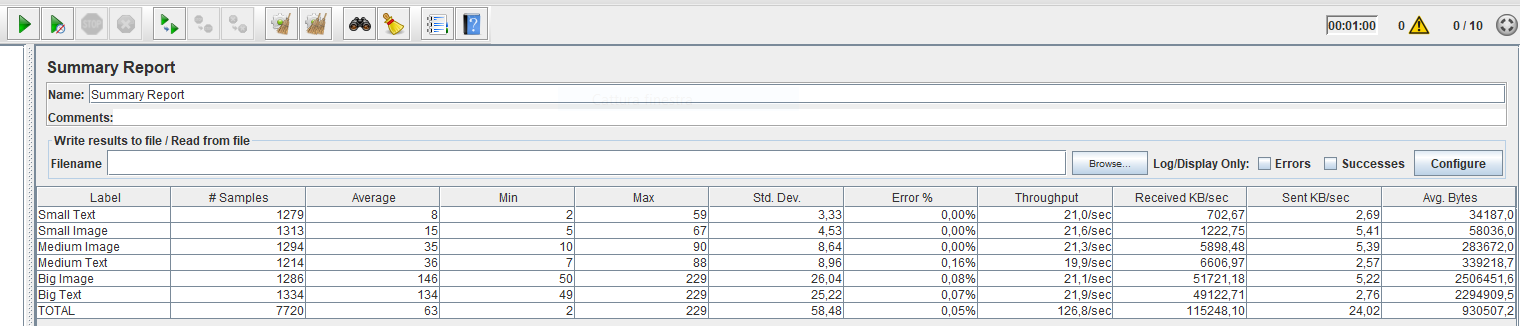
\includegraphics[width=\linewidth]{jmeter_analisi_10thread}
    \end{figure}
  \end{minipage}
  \begin{minipage}{1\linewidth}
    \begin{figure}[H]
      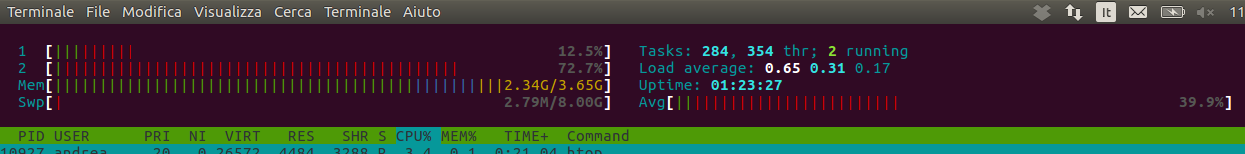
\includegraphics[width=\linewidth]{100_thread_server}
    \end{figure}
  \end{minipage}
\end{minipage}

\subsubsection{Esperimento con 100 Thread Group}
\begin{minipage}{\linewidth}
  \centering
  \begin{minipage}{1\linewidth}
    \begin{figure}[H]
      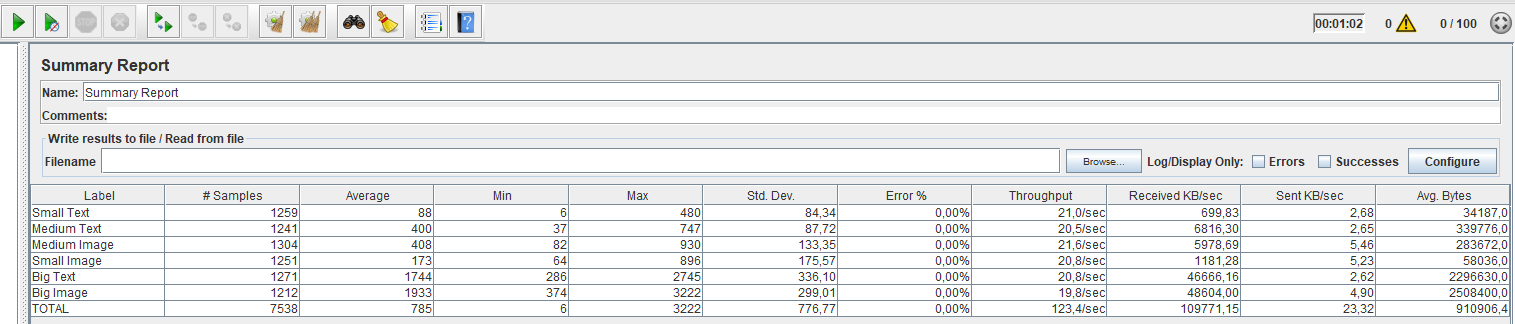
\includegraphics[width=\linewidth]{jmeter_analisi_100thread}
    \end{figure}
  \end{minipage}
  \begin{minipage}{1\linewidth}
    \begin{figure}[H]
      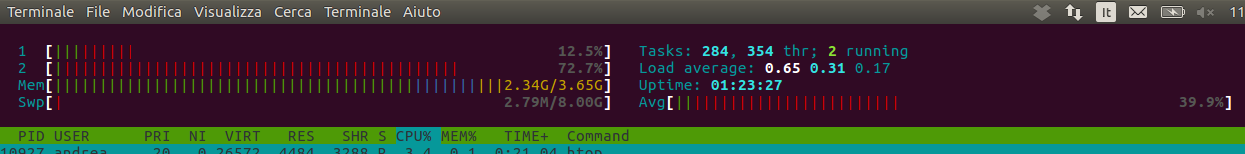
\includegraphics[width=\linewidth]{100_thread_server}
    \end{figure}
  \end{minipage}
\end{minipage}

\subsubsection{Esperimento con 500 Thread Group}
\begin{minipage}{\linewidth}
  \centering
  \begin{minipage}{1\linewidth}
    \begin{figure}[H]
      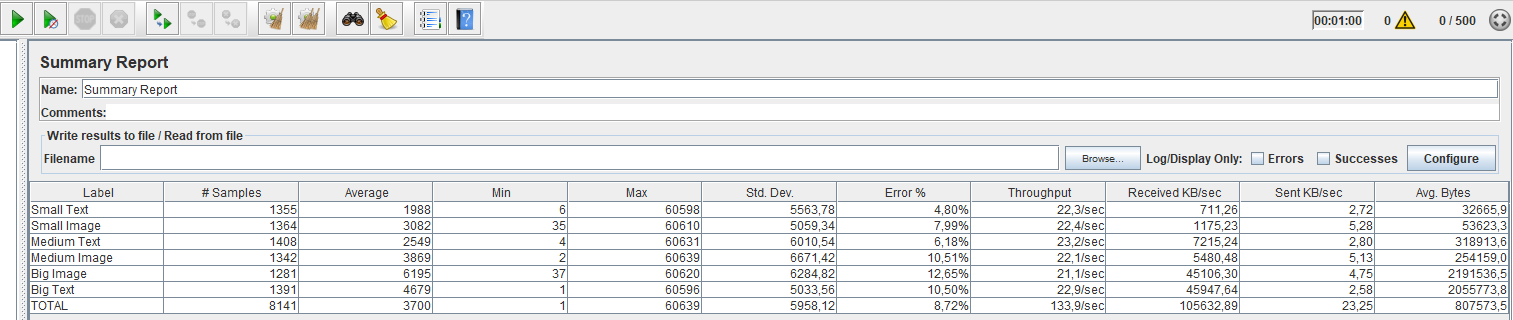
\includegraphics[width=\linewidth]{jmeter_analisi_500thread}
    \end{figure}
  \end{minipage}
  \begin{minipage}{1\linewidth}
    \begin{figure}[H]
      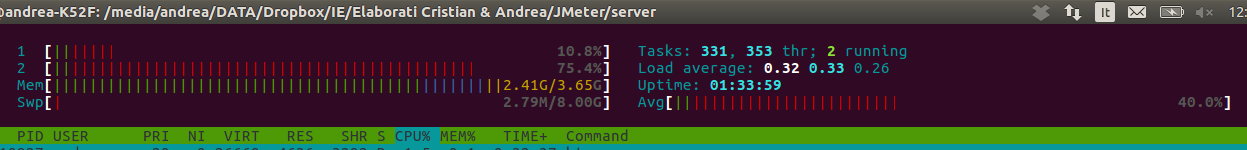
\includegraphics[width=\linewidth]{500_thread_server}
    \end{figure}
  \end{minipage}
\end{minipage}

\subsubsection{Esperimento con 1000 Thread Group}
\begin{minipage}{\linewidth}
  \centering
  \begin{minipage}{1\linewidth}
    \begin{figure}[H]
      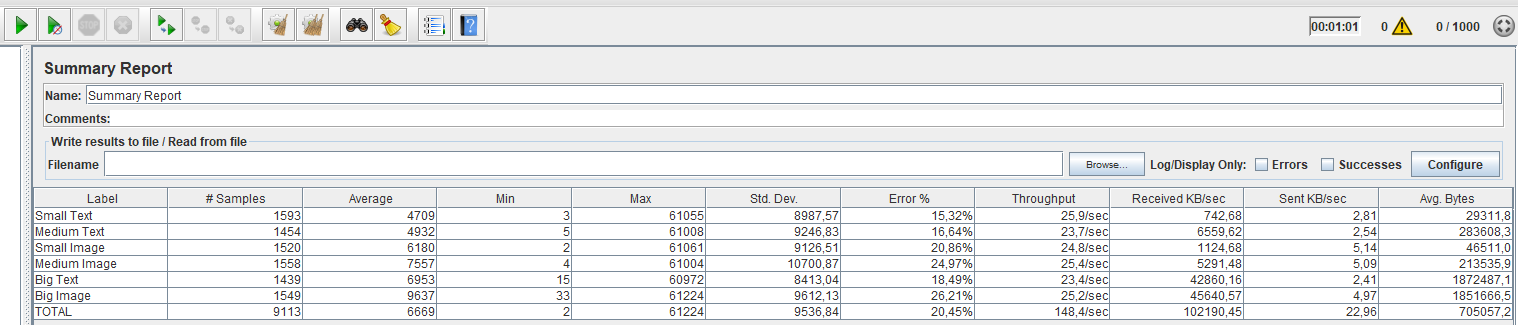
\includegraphics[width=\linewidth]{jmeter_analisi_1000thread}
    \end{figure}
  \end{minipage}
  \begin{minipage}{1\linewidth}
    \begin{figure}[H]
      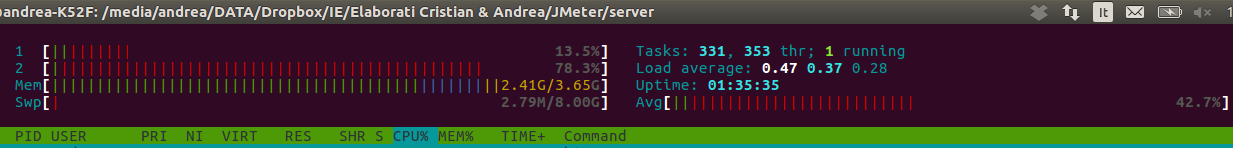
\includegraphics[width=\linewidth]{1000_thread_server}
    \end{figure}
  \end{minipage}
\end{minipage}

\vspace{1cm}
Il parametro Thread Group indica il numero di clients che effettuano continuamente
richieste HTTP al server.\\
Ovviamente questo numero di Threads è simulato dall'unica macchina client utilizzata,
tramite il tool JMeter.\\
Come si può osservare dalle immagini riportate, essendoci una sola macchina fisica,
al crescere del numero di richieste aumenta il numero di errori.\\
Questi errori però non sono da individuare nell'incapacità del server di gestire
la mole di richieste(infatti la CPU è mediamente occupata a circa il 40\% mentre
la RAM al 65\%), bensì nell'infrastruttura di rete(scheda di rete e cavo Ethernet),
limitata ad \textbf{1Gb/s}.\\

In \figurename~\ref{webserver_bottleneck_rete} è riportato l'utilizzo dell'I/O di rete,
raffigurante, in alcuni punti, il raggiungimento del limite fisico(1Gb/s).\\
\begin{figure}[!htbp]
  \centering
  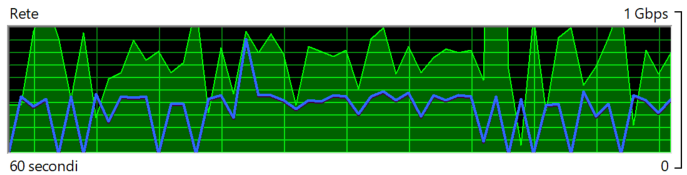
\includegraphics[width=1\linewidth, keepaspectratio]{client_rete_bottleneck}
  \caption{Infrastruttura di Rete - Bottleneck}
  \label{webserver_bottleneck_rete}
\end{figure}

\clearpage

\subsection{Analisi Alto Livello (Client)}
\subsubsection*{Impostazioni Client (JMeter)}
Prima di effettuare gli esperimenti, è stato necessario configurare alcuni parametri
nel Test Plan di JMeter, riportati in \figurename~\ref{webserver_conf_jmeter}

\begin{figure}[!htbp]
  \centering
  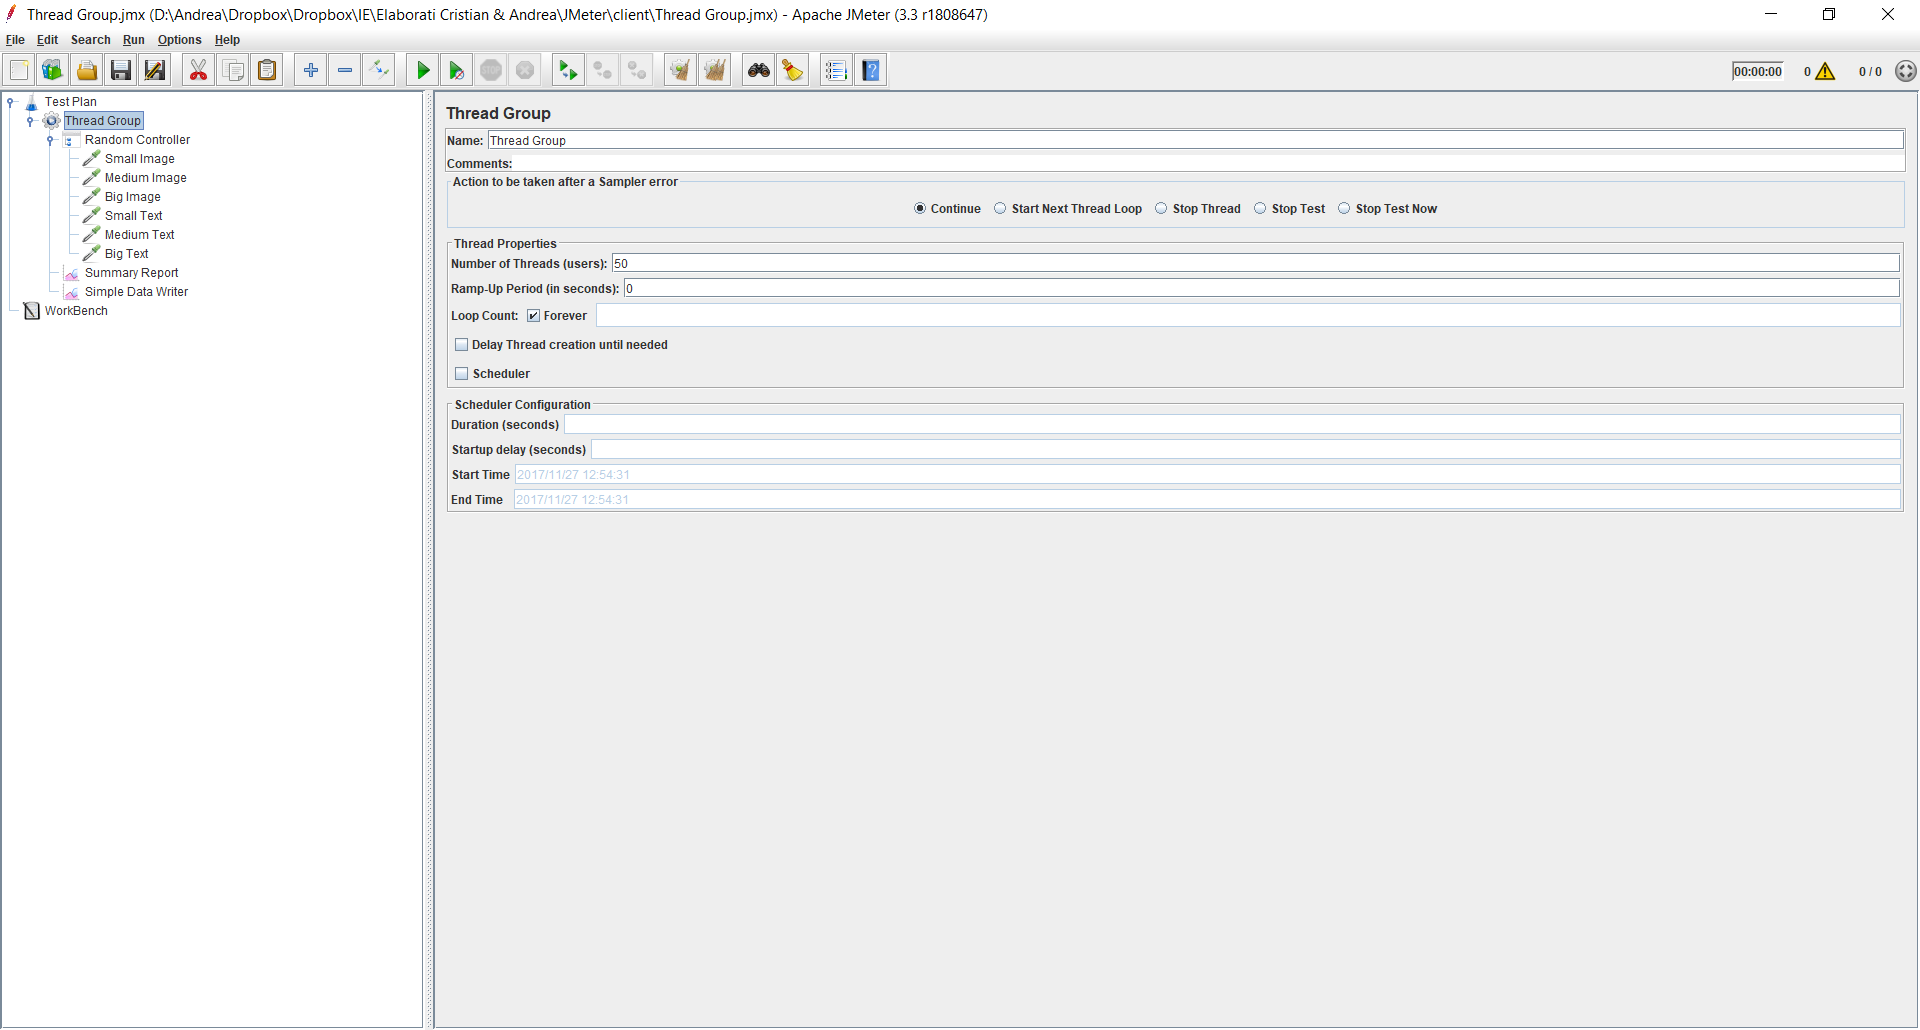
\includegraphics[width=1\linewidth, keepaspectratio]{conf_thread_group}
  \caption{}
  \label{webserver_conf_jmeter}
\end{figure}

In particolare, si evince che il Test Plan è stato caratterizzato dai seguenti
componenti:

\begin{itemize}
  \item \textbf{\textit{Random Controller}} - per generare richieste tra le possibili
  pagine in maniera randomica ed uniforme;
  \item \textbf{\textit{HTTP Request}} - una per pagina, serve per generare una
  richiesta HTTP;
  \item \textbf{\textit{Summary Report}} - genera un report immediato degli esperimenti
  in esecuzione.
  \item \textbf{\textit{Simple Data Writer}} - scrive i risultati degli esperimenti
  in un file .csv
\end{itemize}

JMeter è stato configurato attivando il \textbf{Keep Alive} ad ogni pagina
ed il parametro \textbf{Retrieve All Embedded Resources}(necessario per prelevare
le immagini linkate nell'html).\\
Nonostante gli esperimenti siano stati eseguiti per un tempo di 8 minuti, è stato
effettuato un filtraggio dei dati del primo ed ultimo minuto di esecuzione, al fine
di eliminare eventuali comportamenti transitivi.\\

I parametri utilizzati per la caratterizzazione del workload lato client sono:
\textbf{Latency}, \textbf{Elapsed Time}, \textbf{Bytes}.\\

In \figurename~\ref{webserver_distribuzioni_parametri} sono riportate le distribuzioni dei
tre parametri.\\

\begin{figure}[!htbp]
  \centering
  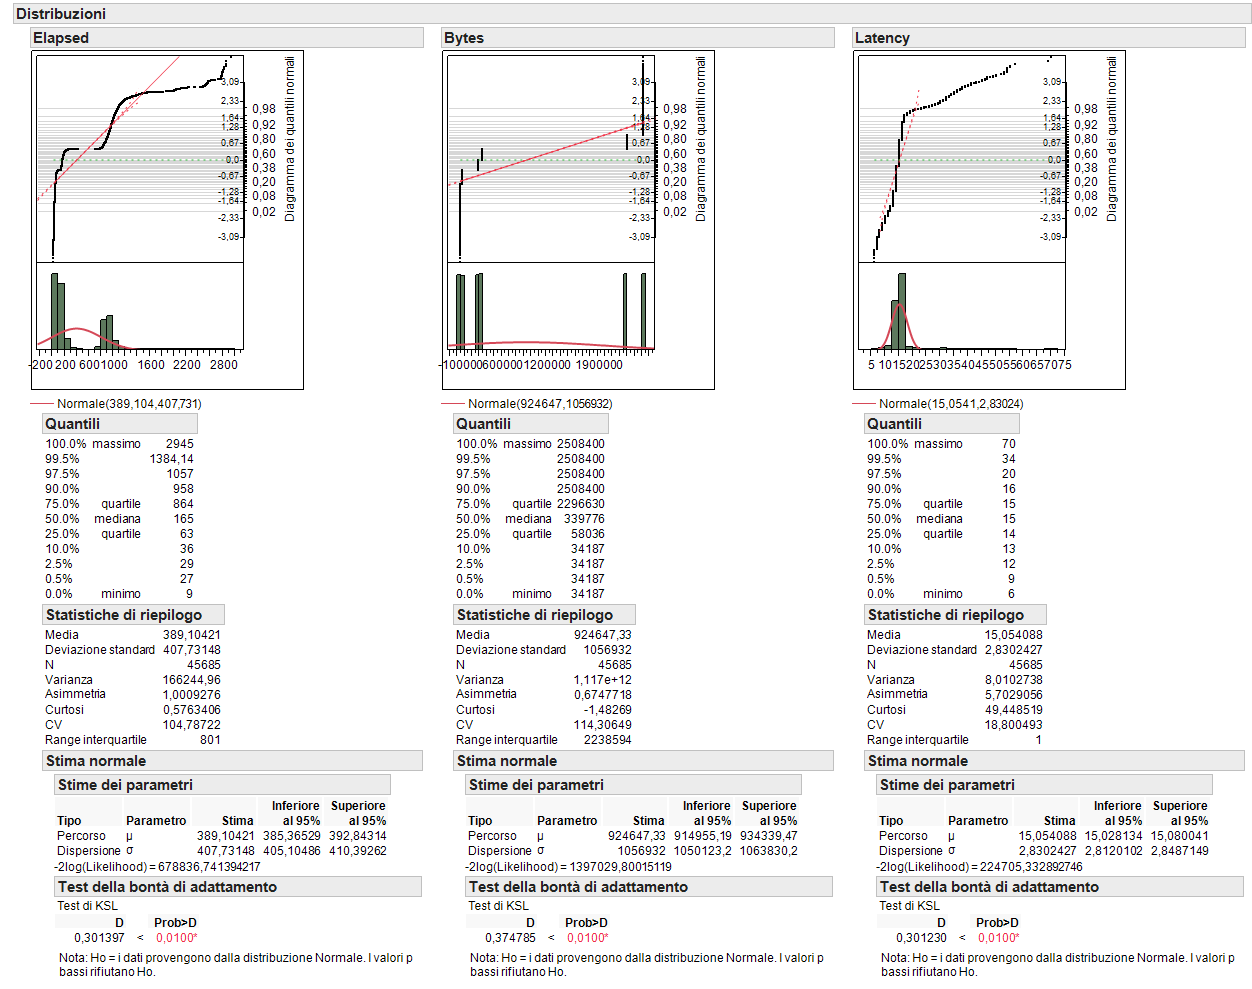
\includegraphics[width=1\linewidth, keepaspectratio]{distribuzioni_client}
  \caption{}
  \label{webserver_distribuzioni_parametri}
\end{figure}

Come si può osservare dal plot Q-Q e dal test di bontà di adattamento, le distribuzioni
non sono normali, di conseguenza, si scelgono \textit{mediana}, come indice di
tendenza centrale e \textit{SIQR}, come indice di dispersione.\\

\begin{center}
  \begin{tabular}{c|c|c|c|}
    & \textbf{Latency} & \textbf{Elapsed Time} & \textbf{Bytes} \\
    \hline
    \textbf{Mediana} & 15 & 165 & 339776 \\
    \hline
    \textbf{SIQR} & 1 & 801 & 2238594 \\
    \hline
  \end{tabular}
\end{center}

\subsubsection*{Correlazione Parametri}
Nella seguente fase vengono studiate possibili correlazioni presenti tra i tre
parametri considerati.\\
Per studiare la correlazione, non volendo fare assunzioni sulla natura delle
distribuzioni, è possibile svolgere il test non parametrico di \textbf{Kendall}.\\
Tale test assume come ipotesi nulla l'indipendenza dei fattori.\\
In particolare, si è interessati ad osservare eventuali correlazioni tra la Latency
e l'Elapsed Time, in \figurename~\ref{webserver_correlazione_elapsed_latency}.\\
\begin{figure}[!htbp]
  \centering
  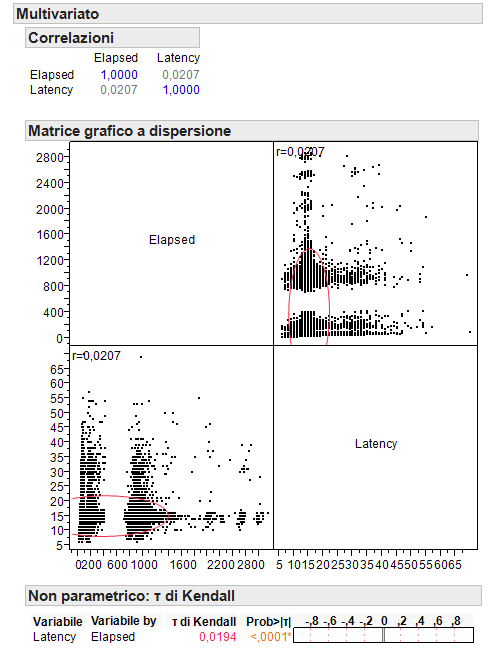
\includegraphics[width=.7\linewidth, keepaspectratio]{correlazione_elapsed_latency}
  \caption{Test di Kendall tra i parametri Elapsed Time e Latency}
  \label{webserver_correlazione_elapsed_latency}
\end{figure}

In questo caso, il test di Kendall suggerisce che l'ipotesi di indipendenza è
rigettata, quindi esiste una forte dipendenza tra i parametri \textit{Latency} e
\textit{Elapsed Time}.

\subsection{Analisi Basso Livello (Server)}
Al fine di misurare il comportamento del server durante l'esperimento, si è
utilizzato il tool \textbf{collectl} simultaneamente all'avvio delle richieste
da parte del client.\\
Il comando lanciato nella bash \textit{Linux} è stato:\\
\begin{center}
  \textbf{collectl -oT -scdmn -P --sep ,}
\end{center}
in particolare:

\begin{itemize}
  \item \textbf{-oT}: aggiunge il timestamp;
  \item \textbf{-scdmn}:  permette di selezionare le periferica di cui si desidera
   monitorare i parametri di performance;
  \item \textbf{-P}: raggruppa i dati su una singola riga;
  \item \textbf{--sep ,}: utilizza la virgola come carattere separatore dei dati.
\end{itemize}

La \textbf{collectl} effettua una misurazione ogni secondo, in accordo al client
che monitora lo stato e le performance delle richieste effettuate.\\
Al fine di eliminare eventuali comportamenti anomali transitivi, l'esperimento è
stato condotto per 8 minuti, eliminando il primo e l'ultimo minuto.\\

Di seguito sono riportati i parametri considerati:
\begin{itemize}
  \item \textbf{CPU}:
  \begin{itemize}
    \item \textbf{\textit{Tot\%}}: percentuale di utilizzo della CPU;
    \item \textbf{\textit{Idle\%}}: percentuale di idle della CPU;
    \item \textbf{\textit{Interpt/sec}}: numero di interrupt al secondo;
    \item \textbf{\textit{Ctx/sec}}: numero di context switch al secondo.
  \end{itemize}
  \item \textbf{Disco}:
  \begin{itemize}
    \item \textbf{\textit{Reads}}: numero di letture al secondo;
    \item \textbf{\textit{RKBytes}}: KiloByte letti;
    \item \textbf{\textit{Writes}}: numero di scritture al secondo;
    \item \textbf{\textit{WKBytes}}: KiloByte scritti.
  \end{itemize}
  \item \textbf{RAM}:
  \begin{itemize}
    \item \textbf{\textit{Used}}: quantità di RAM fisica utilizzata;
    \item \textbf{\textit{Free}}: quantità di RAM fisica libera;
    \item \textbf{\textit{Buffered}}: quanti di RAM fisica utilizzata
    per bufferizzare file;
    \item \textbf{\textit{Cached}}: quantità di RAM fisica utilizzata come memoria cache;
    \item \textbf{\textit{Slab}}: quantità di memoria utilizzata dal kernel come cache per
    le strutture dati, per utilizzo proprio;
    \item \textbf{\textit{Map}}: quantità di memoria utilizzata
    per mappare dispositivi, file o librerie, tramite il comando mmap.
  \end{itemize}
  \item \textbf{Rete}
  \begin{itemize}
    \item \textbf{\textit{RxPkt}}: pacchetti ricevuti;
    \item \textbf{\textit{TxPkt}}: pacchetti trasmessi;
    \item \textbf{\textit{RxKB}}: KiloByte ricevuti;
    \item \textbf{\textit{TxKB}}: KiloByte inviati.
  \end{itemize}
\end{itemize}

Per la caratterizzazione del workload sono state utilizzate le tecniche di PCA e
Clustering.\\
\clearpage
\subsubsection{PCA}
Prima di applicare la PCA è stato analizzato l'andamento temporale dei parametri.\\
Quest'ultimo ha suggerito l'eliminazione dei parametri riguardanti il disco, dal
momento che, avendo eliminato il transitorio(primo ed ultimo minuto), il disco
non effettua alcuna operazione di lettura e/o scrittura in seguito a ulteriori
richieste http.\\
L'unico istante di tempo in cui il disco effettua una lettura è all'inizio
della sessione di test, in cui i dati relativi alle pagine sono caricati in RAM.\\
Nella seguente figura è riportato il primo minuto di test,
durante il quale si osserva un picco letture, con una notevole crescita della
memoria RAM utilizzata.\\

\begin{figure}[!htbp]
  \centering
  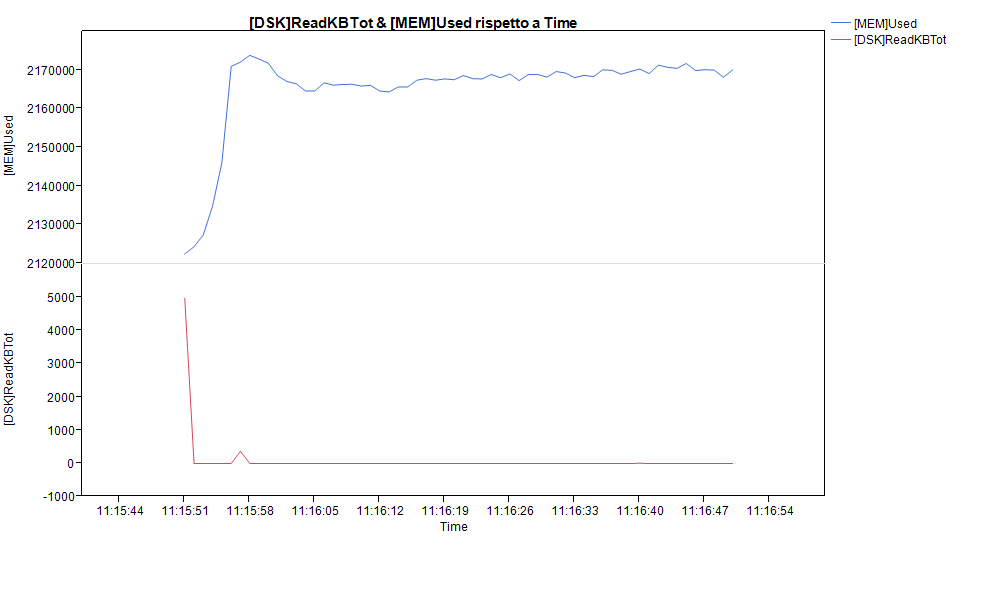
\includegraphics[width=\linewidth, keepaspectratio]{transitorio}
  \caption{Transitorio RAM/DISCO}
  \label{webserver_transitorio}
\end{figure}

\clearpage

Un'ulteriore analisi è stata fatta sul coefficiente di variazione,
per stabilire la presenza di parametri trascurabili, con \textit{CV} nullo.\\
Di seguito è riportato il coefficiente di variazione per ogni parametro.\\

\begin{figure}[!htbp]
  \centering
  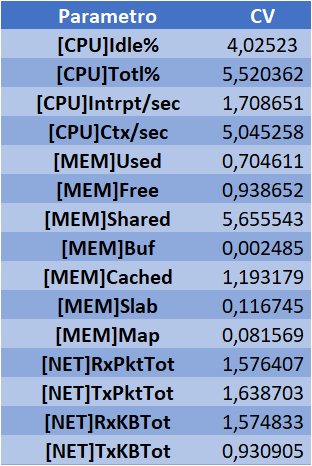
\includegraphics[width=.4\linewidth, keepaspectratio]{cv}
  \caption{CV parametri CPU e RAM}
  \label{webserver_cv1}
\end{figure}
\clearpage
Sfortunatamente non è stato possibile eliminare alcun parametro, poiché non
presentano CV nullo, quindi è stata applicata direttamente la PCA all'intero
workload reale.\\
In \figurename~\ref{webserver_pca} è riportata il risultato ottenuto in JMP.\\

\begin{figure}[!htbp]
  \centering
  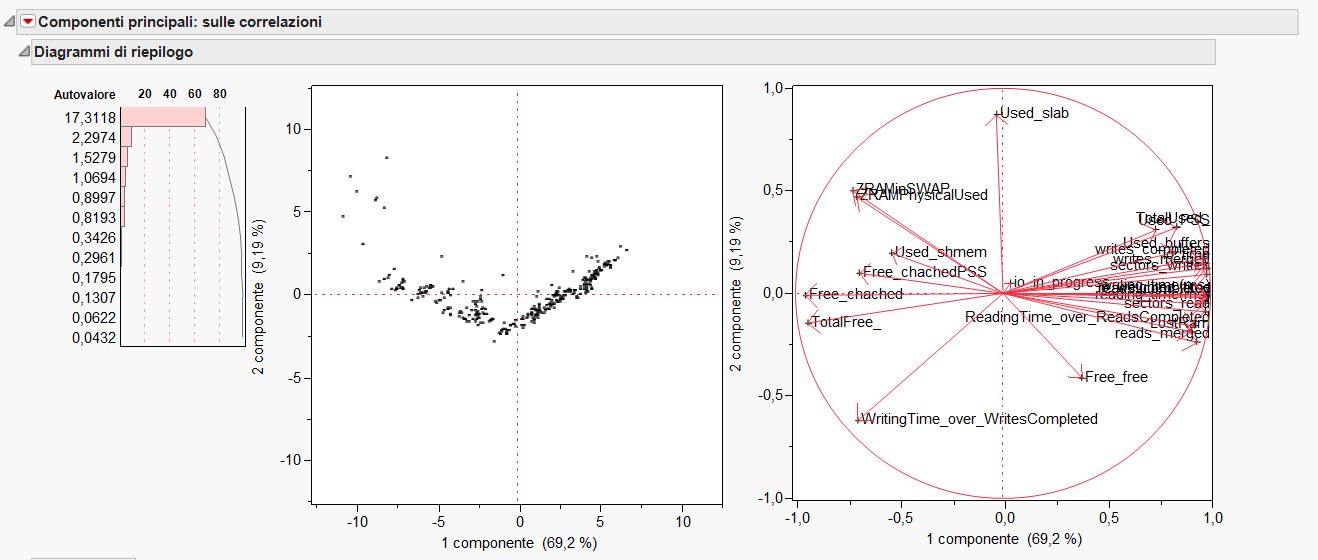
\includegraphics[width=1\linewidth, keepaspectratio]{pca}
  \caption{PCA}
  \label{webserver_pca}
\end{figure}

\begin{figure}[!htbp]
  \centering
  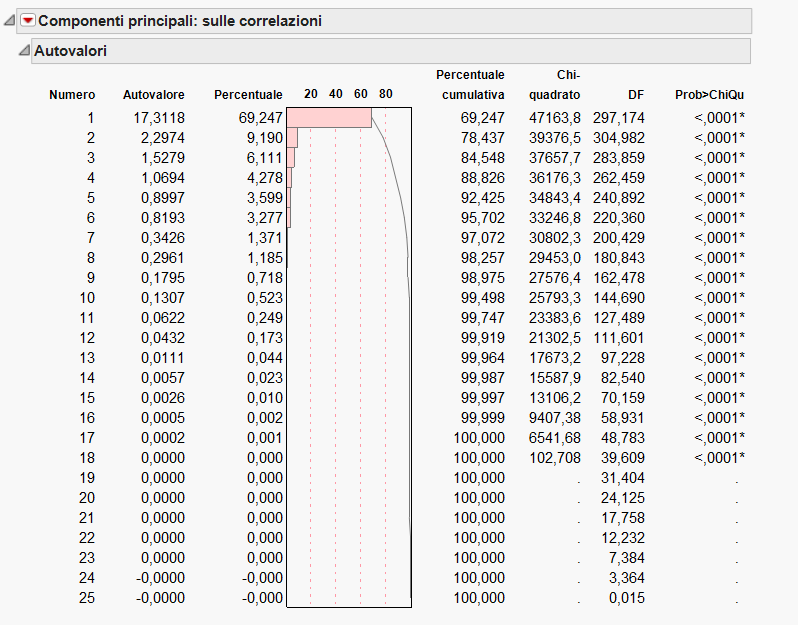
\includegraphics[width=1\linewidth, keepaspectratio]{autovalori}
  \caption{Autovalori PCA}
  \label{webserver_autovalori}
\end{figure}
\clearpage

\begin{figure}[!htbp]
  \centering
  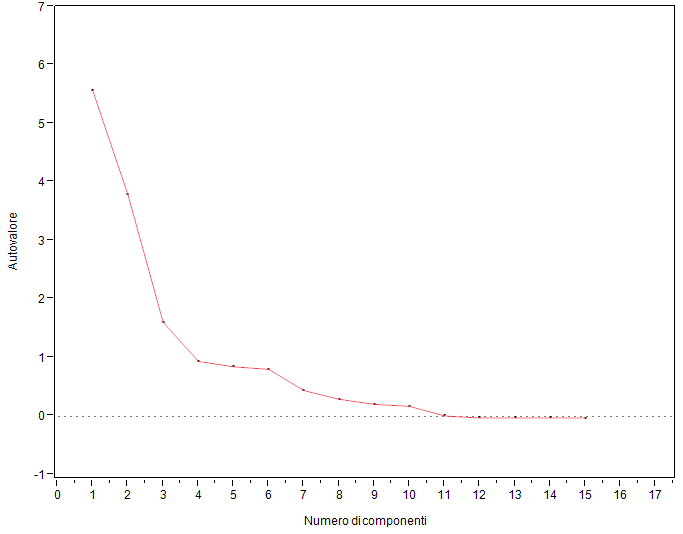
\includegraphics[width=.8\linewidth, keepaspectratio]{scree_pca}
  \caption{Grafico Scree}
  \label{webserver_scree_pca}
\end{figure}

Osservando le Figure \ref{webserver_autovalori} e \ref{webserver_scree_pca} si è scelto di considerare
7 componenti principali conservando il 94,680\% di varianza.

\clearpage

\subsubsection{Clustering}
Dopo aver scelto il numero di componenti principali è stato applicato il clustering
per ridurre il numero di righe del workload reale.\\
In \figurename~\ref{webserver_clustering} è riportato il dendrogramma risultante dal
clustering gerarchico con la relativa curva di clustering, ottenuta in JMP.\\

\begin{figure}[!htbp]
  \centering
  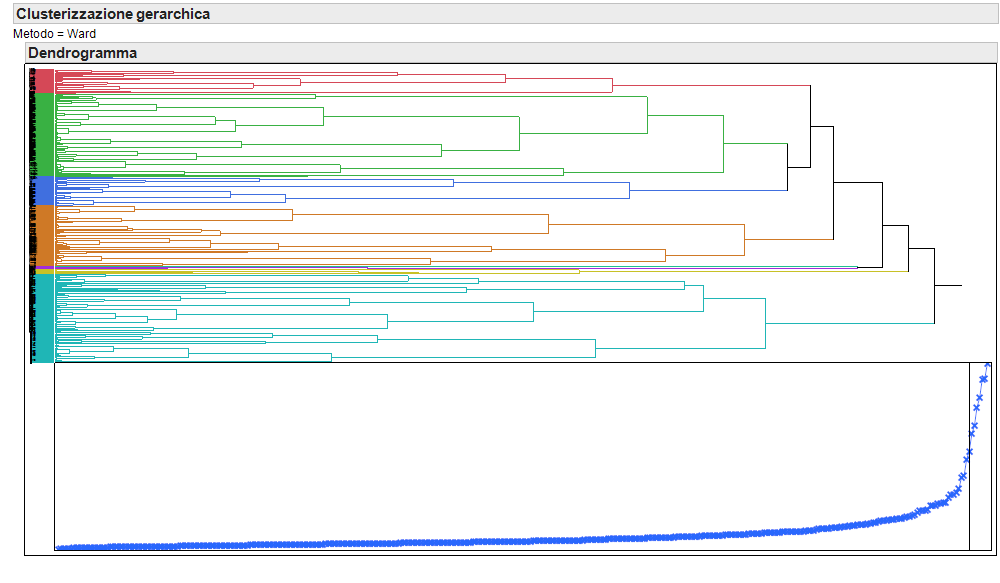
\includegraphics[width=1\linewidth, keepaspectratio]{clustering}
  \caption{Clustering}
  \label{webserver_clustering}
\end{figure}
\clearpage

Osservando le figure \ref{webserver_clustering},
Infatti aggiungendo un ulteriore cluster, il guadagno ottenuto, in termini di varianza,
sarebbe stato trascurabile.\\

\begin{minipage}{\linewidth}
  \centering
  \begin{minipage}{0.48\linewidth}
    \begin{figure}[H]
      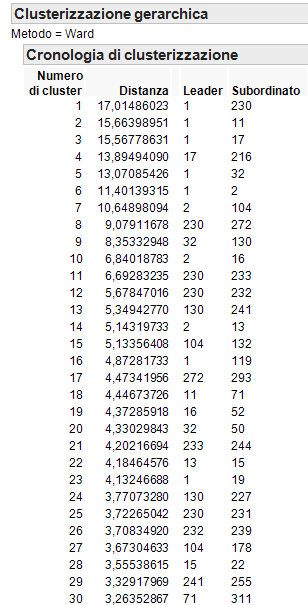
\includegraphics[width=0.9\linewidth]{gerarchia_cluster}
    \end{figure}
  \end{minipage}
  \begin{minipage}{0.48\linewidth}
    \begin{figure}[H]
      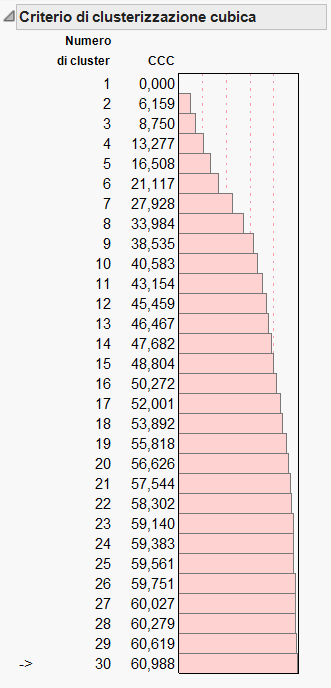
\includegraphics[width=.9\linewidth]{ccc}
    \end{figure}
  \end{minipage}
\end{minipage}
\captionof{figure}{Gerarchia di clustering e Criterio di Clusterizzazione Cubica}
\label{webserver_clustering}

\clearpage

\subsubsection{Caratterizzazione Cluster}
Per caratterizzare ogni cluster, ovvero per individuare quale stato del sistema
esso rappresentasse, sono state analizzate le figure \ref{webserver_autovettori}, \ref{webserver_graph}
e \ref{webserver_cluster_time}.\\
La figura \ref{webserver_autovettori} mostra gli autovettori delle 7 componenti principali,
dai quali è facile individuare i parametri del workload reale che maggiormente
incidono su ognuna di esse.\\
\begin{figure}[!htbp]
  \centering
  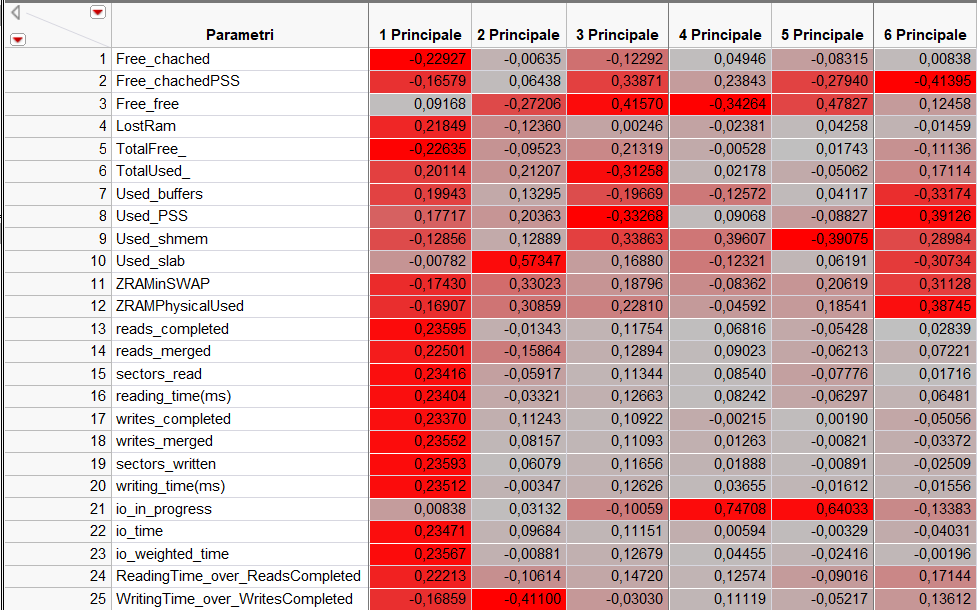
\includegraphics[width=.9\linewidth, keepaspectratio]{autovettori}
  \caption{Autovettori PCA}
  \label{webserver_autovettori}
\end{figure}

In particolare:

\begin{itemize}
  \item \textbf{\textit{Principale 1}}: influenzata maggiormente da parametri
  riguardanti la RAM.\\
  Nello specifico si nota che \textit{Used} e \textit{Free} si comportano in maniera duale;
  \item \textbf{\textit{Principale 2}}: influenzata maggiormente dai parametri
  di rete, \textit{Intrpt/sec} e \textit{Idle\%};
  \item \textbf{\textit{Principale 3}}: influenzata da \textit{Totl\%} e \textit{Idle\%};
  \item \textbf{\textit{Principale 4}}: influenzata da \textit{Map} e \textit{TxPktTot};
  \item \textbf{\textit{Principale 5}}: influenzata da \textit{Ctx/sec} e \textit{TxPktTot};
  \item \textbf{\textit{Principale 6}}: influenzata da \textit{Ctx/sec}, \textit{Map},
  \textit{RxPktTot}, \textit{TxPktTot} e \textit{RxKBTot};
  \item \textbf{\textit{Principale 7}}: influenzata da \textit{Buf} e \textit{Slab};
\end{itemize}

\clearpage

La figura \ref{webserver_graph} mostra quali sono le componenti principali che hanno contribuito
maggiormente alla creazione dei cluster.\\

\begin{figure}[!htbp]
  \centering
  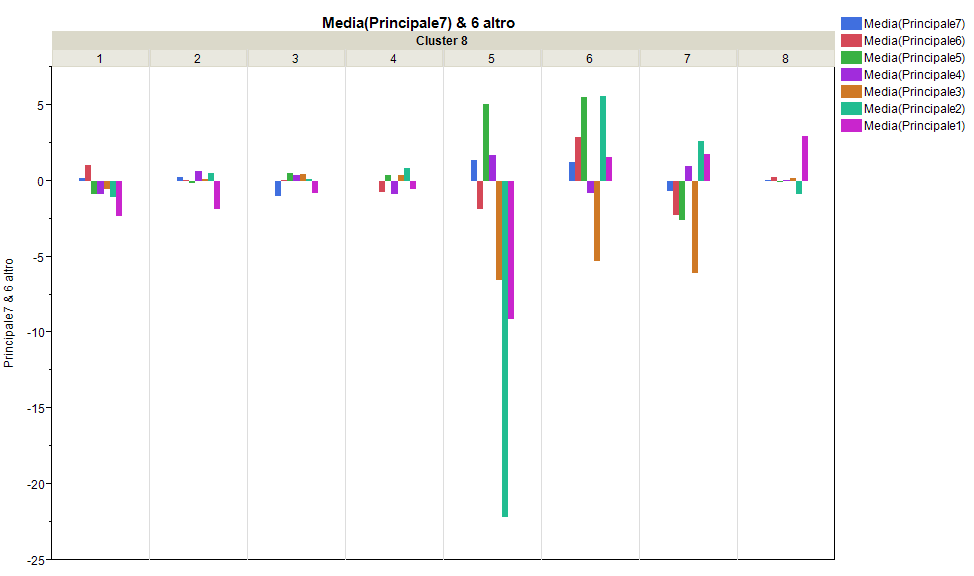
\includegraphics[width=0.8\linewidth, keepaspectratio]{graph}
  \caption{}
  \label{webserver_graph}
\end{figure}
La figura \ref{webserver_cluster_time} mostra la composizione dei cluster rispetto al tempo.\\
\begin{figure}[!htbp]
  \centering
  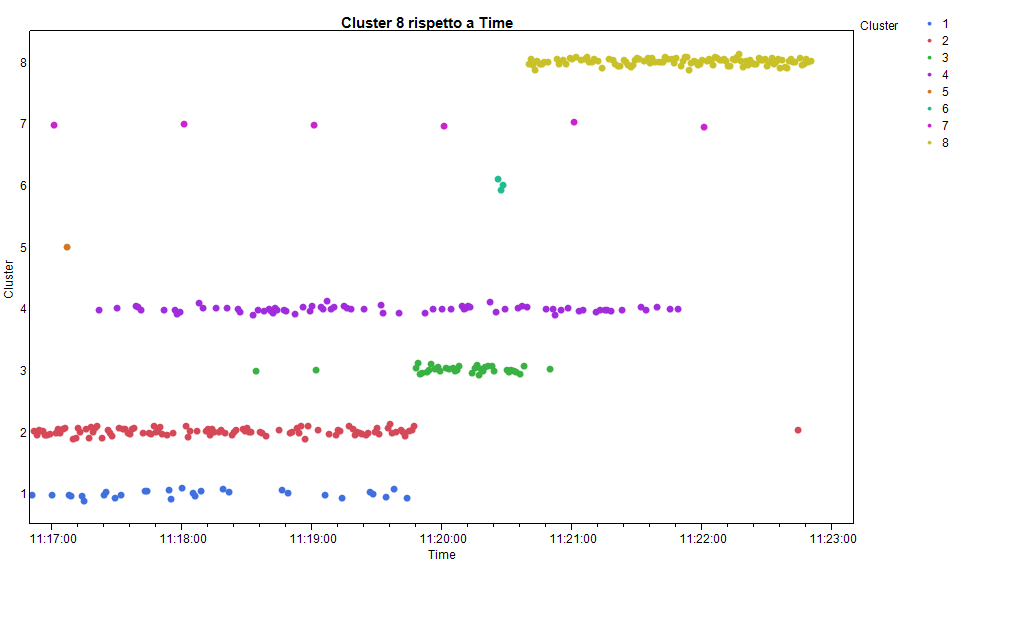
\includegraphics[width=.8\linewidth, keepaspectratio]{cluster_time}
  \caption{}
  \label{webserver_cluster_time}
\end{figure}

\clearpage

Di seguito è riportata la caratterizzazione dei singoli cluster ed una loro
rappresentazione grafica 3D, in funzione di tre componenti principali.\\
In questi grafici i campioni plottati hanno una sfumatura dal blu al rosso, in
funzione del tempo, in cui il blu rappresenta il primo minuto del test ed il
rosso l'ultimo.\\

\begin{itemize}

  \begin{figure}[!htbp]
    \centering
    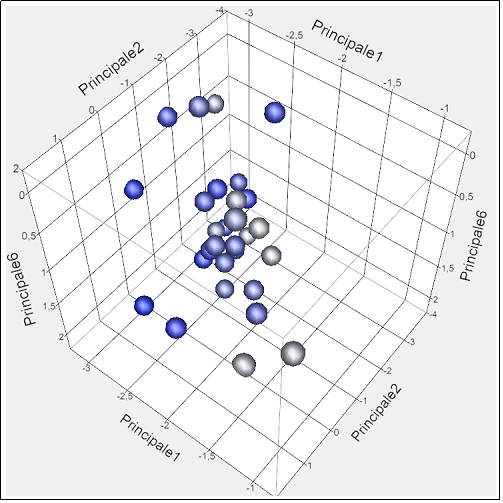
\includegraphics[width=.45\linewidth, keepaspectratio]{cluster1}
    \caption{Grafico 3D del Cluster 1}
    \label{webserver_cluster1}
  \end{figure}

  \item \textbf{Cluster 1}: influenzato maggiormente da valori negativi della
  1 e 2 componente principale e positivi della 6.\\
  In particolare, osservando la figura \ref{webserver_cluster_time} e \ref{webserver_cluster1}, i campioni contenuti
  in questo cluster appartengono alla prima metà dell'esperimento.\\
  Analizzando più approfonditamente la cause della creazione di tale cluster si
  identifica quale stato del sistema esso rappresenta.\\
  A causa di valori negativi della prima componente principale esso
  rappresenta uno stato del sistema con bassa occupazione della memoria RAM,
  in quanto il valore della parametro \textit{Free} nei campioni del cluster 1,
  essendo negativo in corrispondenza della principale 1 in figura \ref{webserver_autovettori},
  fornisce sicuramente un impatto maggiore rispetto agli altri parametri.\\
  Inoltre si può affermare che a causa della seconda componente principale negativa
  l'attività di rete è bassa, in quanto nella figura \ref{webserver_autovettori} si osserva
  che i parametri di rete influenzano positivamente la principale due, di conseguenza
  per assumere valori negativi, i parametri di rete devono assumere valori bassi.

  \clearpage

  \begin{figure}[!htbp]
    \centering
    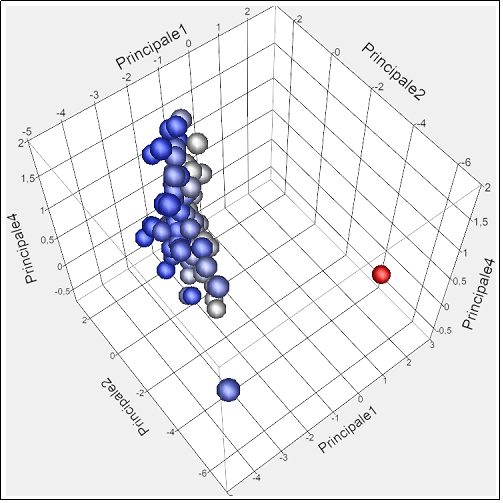
\includegraphics[width=.45\linewidth, keepaspectratio]{cluster2}
    \caption{Cluster 2}
    \label{webserver_cluster2}
  \end{figure}

  \item \textbf{Cluster 2}: influenzato maggiormente da valori negativi della
  1 e positivi della 2 e 4 componente principale.\\
  In particolare, osservando la figura \ref{webserver_cluster_time} e \ref{webserver_cluster1}, i campioni contenuti
  in questo cluster appartengono alla prima metà dell'esperimento.\\
  Analizzando più approfonditamente la cause della creazione di tale cluster si
  identifica quale stato del sistema esso rappresenta.\\
  In particolare il cluster rappresenta uno stato del sistema in cui la quantità di RAM occupata
  è bassa, comportamento verificato nel primo cluster, ma in maniera opposta,
  essendo positiva la principale due e presentando un'attività di rete più intensa.

  \clearpage

  \begin{figure}[!htbp]
    \centering
    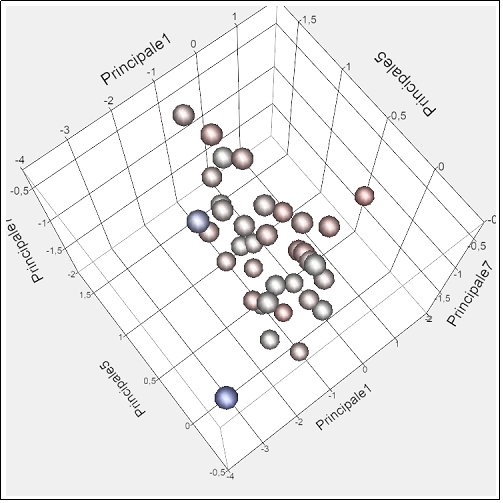
\includegraphics[width=0.45\linewidth, keepaspectratio]{cluster3}
    \caption{Cluster 3}
    \label{webserver_cluster3}
  \end{figure}

  \item \textbf{Cluster 3}: influenzato maggiormente da valori negativi della
  1 e 7 principale, e positivi della 5.\\
  In particolare, osservando la figura \ref{webserver_cluster_time} e \ref{webserver_cluster1}, i campioni contenuti
  in questo cluster appartengono ad un intervallo temporale centrale dell'esperimento.\\
  Analizzando più approfonditamente la cause della creazione di tale cluster si
  identifica quale stato del sistema esso rappresenta.\\
  In particolare il cluster rappresenta uno stato in cui la quantità di RAM occupata
  è bassa, comportamento verificato nel primo cluster, con attività di rete in trasmissione
  bassa e aumento delle memoria RAM dedicata al buffering dei file.

  \clearpage

  \begin{figure}[!htbp]
    \centering
    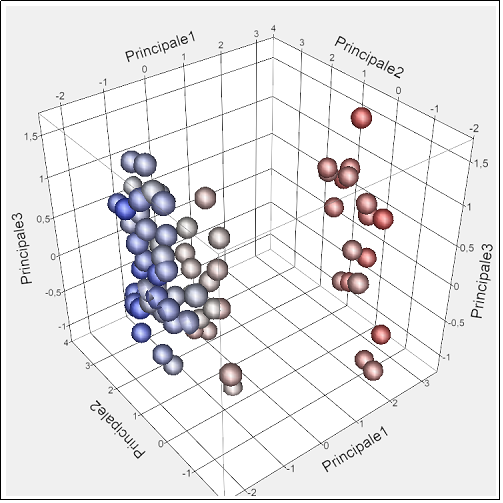
\includegraphics[width=.45\linewidth, keepaspectratio]{cluster4}
    \caption{Cluster 4}
    \label{webserver_cluster4}
  \end{figure}

  \item \textbf{Cluster 4}: presenta valori delle componenti principali per cui non
  è possibile una corretta caratterizzazione.\\
  Per poter essere ugualmente analizzato, il cluster è stato suddiviso in due
  sotto-cluster, utilizzando la cronologia di clusterizzazione mostrata in
  precedenza.\\
  In figura \ref{webserver_cluster_4_diviso} è riportata l'incidenza delle componenti
  principali sui due sotto-cluster.\\

  \begin{figure}[!htbp]
    \centering
    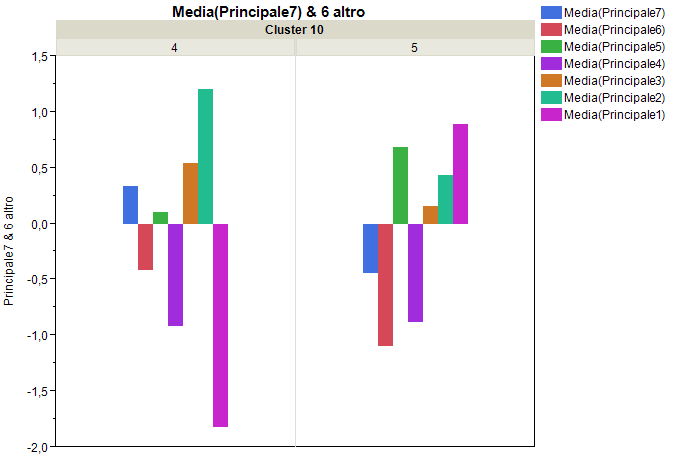
\includegraphics[width=.6\linewidth, keepaspectratio]{cluster_4_diviso}
    \caption{}
    \label{webserver_cluster_4_diviso}
  \end{figure}

  Dalla figura \ref{webserver_cluster_4_diviso} si possono caratterizzare i cluster 4.1 e 4.2.\\
  Il cluster 4.1 risulta influenzato  negativamente dalle principali 1 e 4
  e positivamente dalla principale 2, quindi c'è un alta attività di rete
  e una bassa quantità di memoria RAM occupata.\\
  Il cluster 4.2 risulta influenzato negativamente dalle principali 6 e 4,
  e positivamente dalla principale 1.\\
  Dunque si evince un'alta attività di rete ed un'elevata occupazione di memoria
  RAM.\\

  \begin{figure}[!htbp]
    \centering
    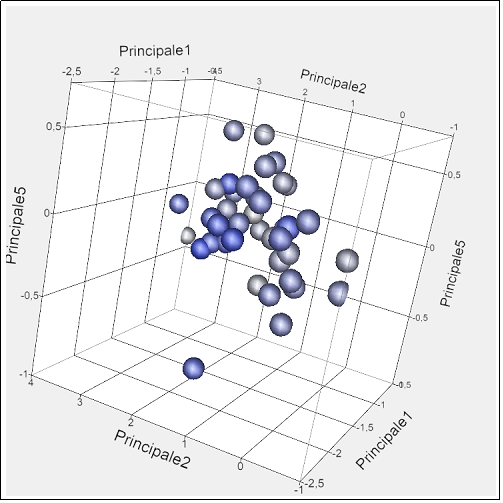
\includegraphics[width=.45\linewidth, keepaspectratio]{cluster41}
    \caption{Cluster 4.1}
    \label{webserver_cluster41}
  \end{figure}

  \begin{figure}[!htbp]
    \centering
    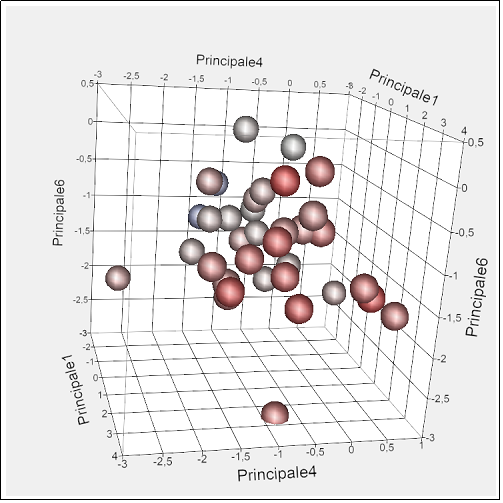
\includegraphics[width=.45\linewidth, keepaspectratio]{cluster42}
    \caption{Cluster 4.2}
    \label{webserver_cluster42}
  \end{figure}

  \clearpage

  \begin{figure}[!htbp]
    \centering
    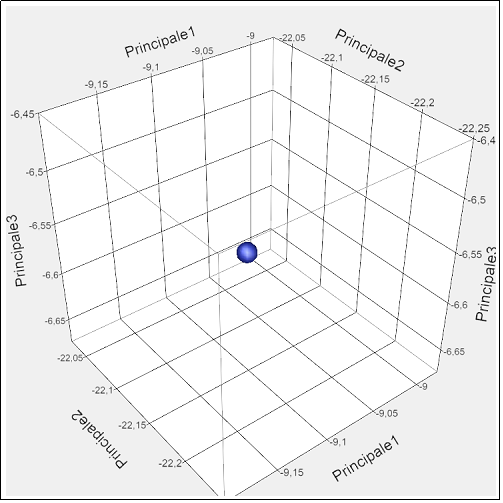
\includegraphics[width=.4\linewidth, keepaspectratio]{cluster5}
    \caption{Cluster 5}
    \label{webserver_cluster5}
  \end{figure}

  \item \textbf{Cluster 5}: tale cluster è formato da un solo campione, essendo
  esso un outlier, necessita di essere analizzato per capire se è possibile eliminarlo.\\
  La creazione di tale cluster è attribuita maggiormente alla principale
  2, condizionata a sua volta dai parametri \textbf{RxPktTot} e \textbf{RxKBTot}.\\
  Analizzando il grafico in figura \ref{webserver_cluster5_temp_analisi}, il quale riporta
  l'andamento temporale di \textbf{RxKBTot}, si osserva che in corrispondenza del
  cluster 5 c'è un picco negativo il quale può essere attribuito ad una riduzione
  della velocità di trasmissione del client.\\
  Quindi è stato deciso di non considerare tale cluster nella fase finale di
  generazione del workload sintetico.\\

  \begin{figure}[!htbp]
    \centering
    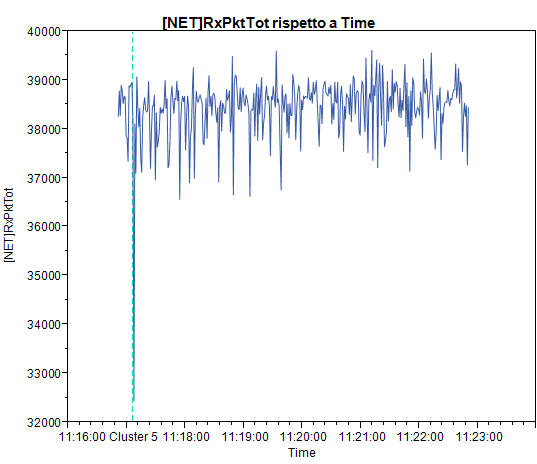
\includegraphics[width=.5\linewidth, keepaspectratio]{cluster5_temp_analisi}
    \caption{Andamento temporale di RxPktTot}
    \label{webserver_cluster5_temp_analisi}
  \end{figure}

  \clearpage

  \begin{figure}[!htbp]
    \centering
    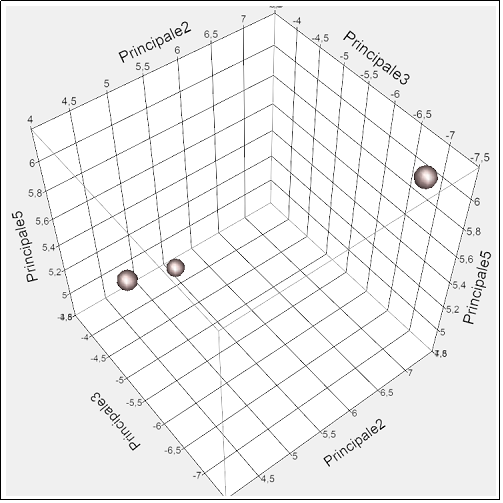
\includegraphics[width=0.45\linewidth, keepaspectratio]{cluster6}
    \caption{Cluster 6}
    \label{webserver_cluster6}
  \end{figure}

  \item \textbf{Cluster 6}: la formazione di tale cluster è attribuita alle
  componenti principali 2,3 e 5, le quali sono state influenzate maggiormente
  da \textit{RxPktTot}, \textit{Tot\%}, \textit{TxPktTot} e \textit{Ctx/s}.\\
  Analizzando la figura \ref{webserver_analisi_temp_cluster_6}, la quale riporta l'andamento
  temporale dei parametri sopra descritti, si nota che tali campioni sono consecutivi
  e individuano un picco di \textit{Ctx/s}, il quale può essere attributo all'esecuzione
  di altri processi presenti nel server.\\
  A tal proposito si può ritenere irrilevante tale cluster ai fini della
  caratterizzazione del workload sintetico.\\

  \begin{figure}[!htbp]
    \centering
    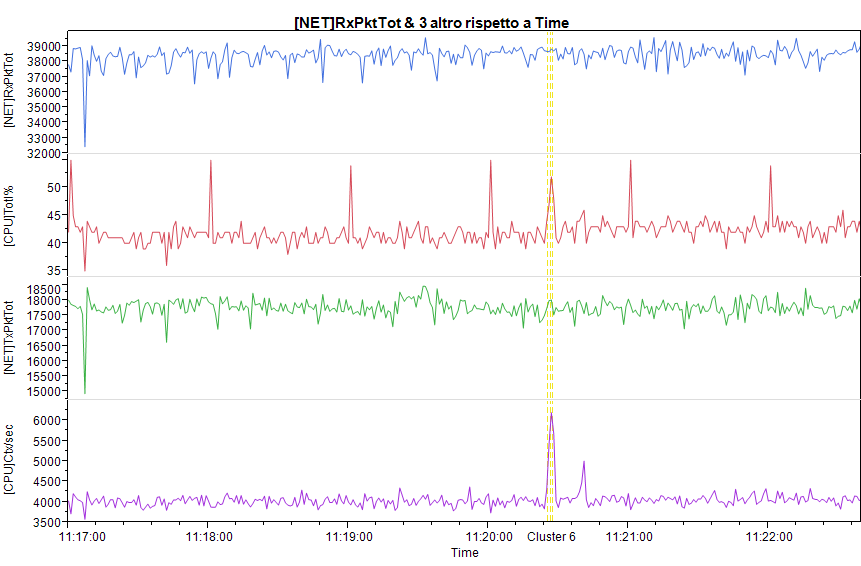
\includegraphics[width=0.6\linewidth, keepaspectratio]{analisi_temp_cluster_6}
    \caption{Analisi temporale \textit{RxPktTot}, \textit{Tot\%}, \textit{TxPktTot} e \textit{Ctx/s}}
    \label{webserver_analisi_temp_cluster_6}
  \end{figure}

  \clearpage

  \begin{figure}[!htbp]
    \centering
    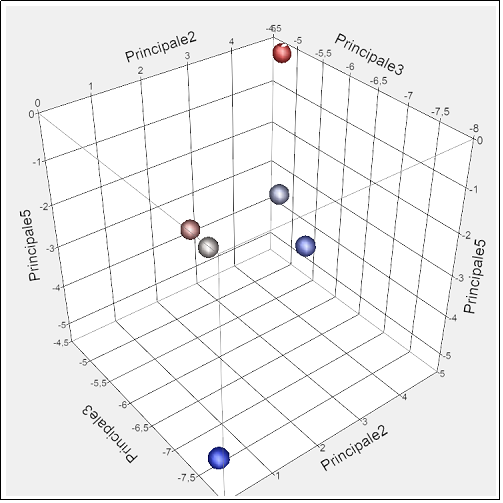
\includegraphics[width=.45\linewidth, keepaspectratio]{cluster7}
    \caption{Cluster 7}
    \label{webserver_cluster7}
  \end{figure}

  \item \textbf{Cluster 7}: la formazione di tale cluster è attribuibile maggiormente
  alla 3 componente principale, la quale è stata influenza dal parametro \textit{Tot\%}.\\
  Analizzando il comportamento temporale di tale parametro, in figura \ref{webserver_analisi_temp_cluster_7},
  si osserva che tale cluster contiene picchi di utilizzo della CPU, ad ogni
  occorrenza del primo secondo di ogni minuto di test.\\
  \'E stato monitorato il sistema server anche in assenza di esecuzione del workload,
  e tale fenomeno ha continuato a manifestarsi, dimostrandosi inerente al
  comportamento del sistema operativo.\\
  Per questo motivo questo cluster non è stato considerato ai fini della
  caratterizzazione del workload sintetico.\\

  \begin{figure}[!htbp]
    \centering
    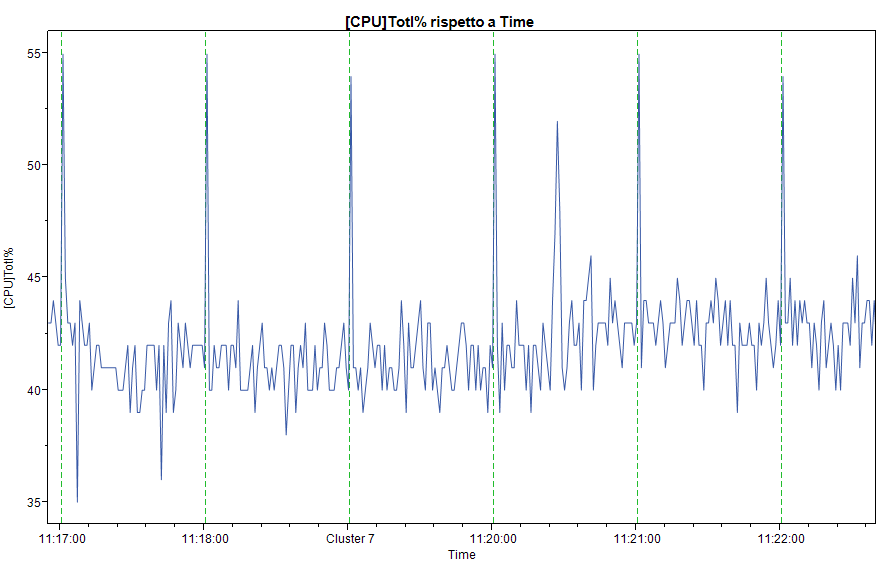
\includegraphics[width=0.6\linewidth, keepaspectratio]{analisi_temp_cluster_7}
    \caption{Analisi temporale \textit{Tot\%}}
    \label{webserver_analisi_temp_cluster_7}
  \end{figure}

  \clearpage

  \begin{figure}[!htbp]
    \centering
    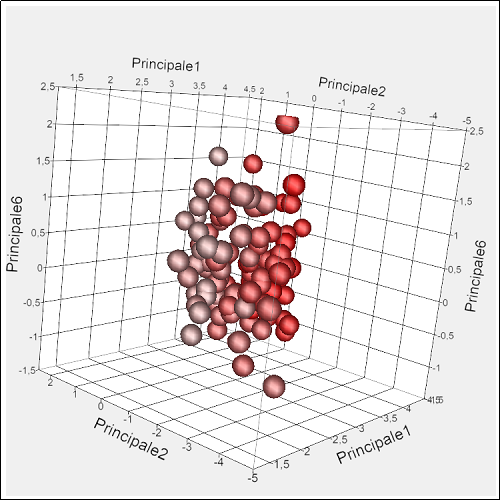
\includegraphics[width=.45\linewidth, keepaspectratio]{cluster8}
    \caption{Cluster 8}
    \label{webserver_cluster8}
  \end{figure}

  \item \textbf{Cluster 8}: rappresenta la parte finale dell'esperimento.\\
  Lo stato del sistema che esso rappresenta è dato da un'elevata occupazione
  di RAM ed una bassa attività di rete, risultando essere il duale del \textit{cluster 1}.\\

\end{itemize}
\clearpage
Scegliendo come punti rappresentanti ogni cluster il loro centroide, il Workload
Sintetico ottenuto è il seguente.
\begin{figure}[!htbp]
  \centering
  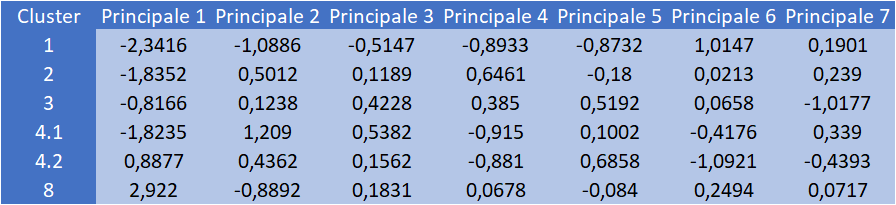
\includegraphics[width=1\linewidth, keepaspectratio]{centroidi}
  \caption{Workload Sintetico}
  \label{webserver_centroidi}
\end{figure}

La percentuale di devianza persa approssimando il workload reale con quello
sintetico è il \textbf{33,27\%}.

\begin{minipage}{\linewidth}
  \centering
  \begin{minipage}{0.48\linewidth}
    \begin{figure}[H]
      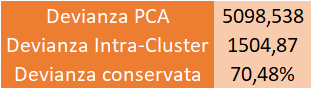
\includegraphics[width=0.9\linewidth]{devianza}
    \end{figure}
  \end{minipage}
  \begin{minipage}{0.48\linewidth}
    \begin{figure}[H]
      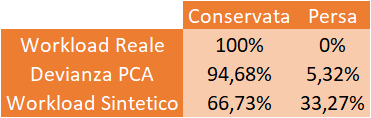
\includegraphics[width=.9\linewidth]{significativita_workload}
    \end{figure}
  \end{minipage}
\end{minipage}

\clearpage

\section{Capacity Test}
Questa sezione è dedicata allo studio della capacità di carico del sistema.\\
Il capacity test è attuato sulla base del workload caratterizzato in precedenza,
in funzione della tipologia di richieste effettuate al server(pagine di
piccola, media e grande dimensione).\\
I parametri di interesse nel capacity test sono le \textit{Richieste al minuto(Req/min)},
il \textit{Throughput} e l'\textit{Elapsed Time}.\\
Il test procede incrementando le Req/min ed osservando i 2 parametri di risposta
del sistema.\\
Plottando i risultati ottenuti è possibile individuare due punti di funzionamento
del sistema, noti come:
\begin{itemize}
  \item \textbf{Knee Capacity} - punto di funzionamento in cui il sistema ha un
  buon throughput e dei tempi di risposta bassi;
  \item \textbf{Usable Capacity} - punto di funzionamento limite in cui il sistema
  ha un ottimo throughput, ma oltre il quale c'è un degrado notevole nelle prestazioni.
\end{itemize}

Per il test effettuato con il tool JMeter, è stato scelto di di simulare 50 Threads
attivi.\\

\subsection{Test pagine HTML piccole}
In questo caso sono state utilizzate esclusivamente le richieste HTTP per le pagine
\textit{small\_text} e \textit{small\_image}.\\
In \figurename~\ref{webserver_small_page_summary_report} sono presenti gli esiti del
Summary Report di JMeter.\\

\begin{figure}[!htbp]
  \centering
  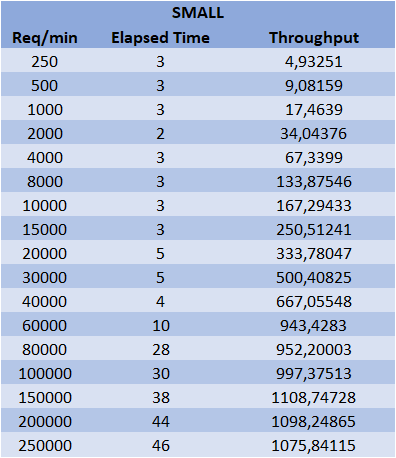
\includegraphics[width=.4\linewidth, keepaspectratio]{capacitytest_small}
  \caption{Test pagine HTML piccole}
  \label{webserver_small_page_summary_report}
\end{figure}

Utilizzando il costruttore di Grafici di \textit{JMP} sono stati analizzati i plot
di Throughput ed Elapsed Time, e definiti i punti di \textit{Knee Capacity} e
\textit{Usable Capacity}.\\

\begin{figure}[!htbp]
  \centering
  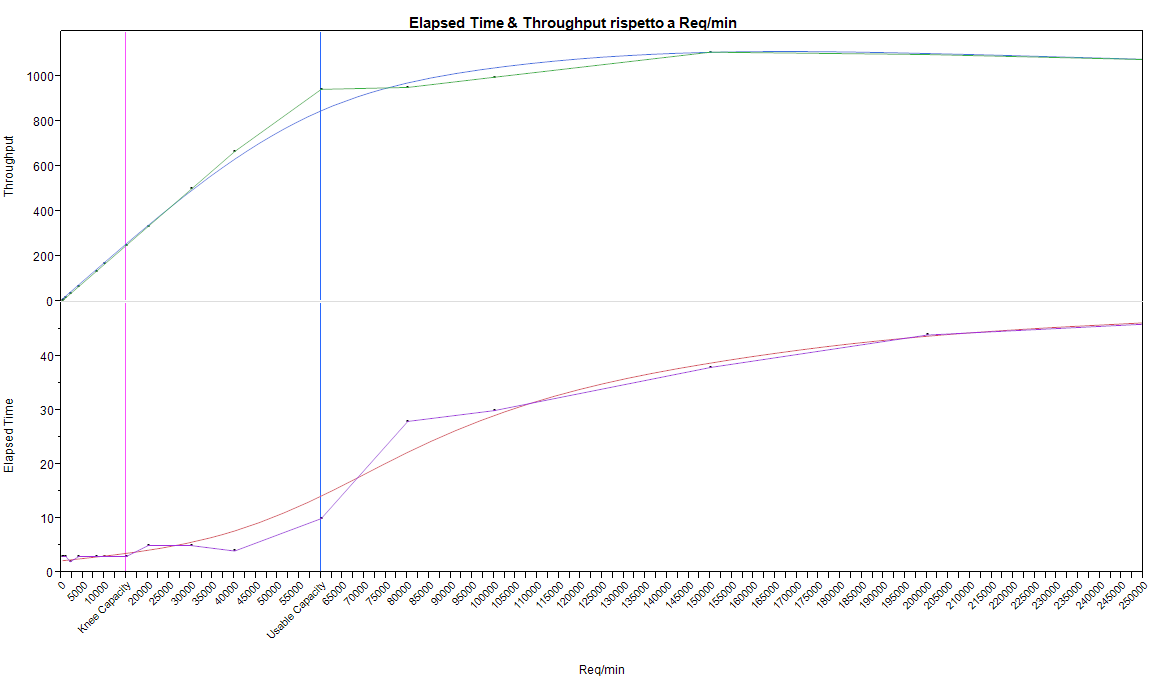
\includegraphics[width=\linewidth, keepaspectratio]{usable_knee_small}
  \caption{Capacity: Knee (15000 Req/min) / Usable (60000 Req/min)}
\end{figure}

\subsection{Test pagine HTML medie}
In questo caso sono state utilizzate esclusivamente le richieste HTTP per le pagine
\textit{medium\_text} e \textit{medium\_image}.\\
In \figurename~\ref{webserver_medium_page_summary_report} sono presenti gli esiti del
Summary Report di JMeter.\\

\begin{figure}[!htbp]
  \centering
  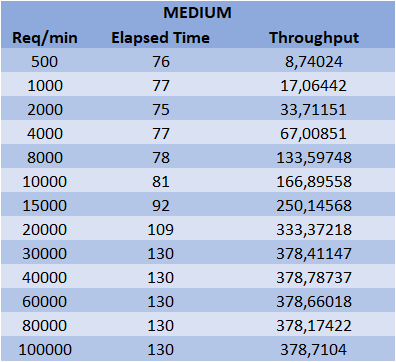
\includegraphics[width=.4\linewidth, keepaspectratio]{capacitytest_medium}
  \caption{Test pagine HTML medie}
  \label{webserver_medium_page_summary_report}
\end{figure}

Utilizzando il costruttore di Grafici di \textit{JMP} sono stati analizzati i plot
di Throughput ed Elapsed Time, e definiti i punti di \textit{Knee Capacity} e
\textit{Usable Capacity}.\\

\begin{figure}[!htbp]
  \centering
  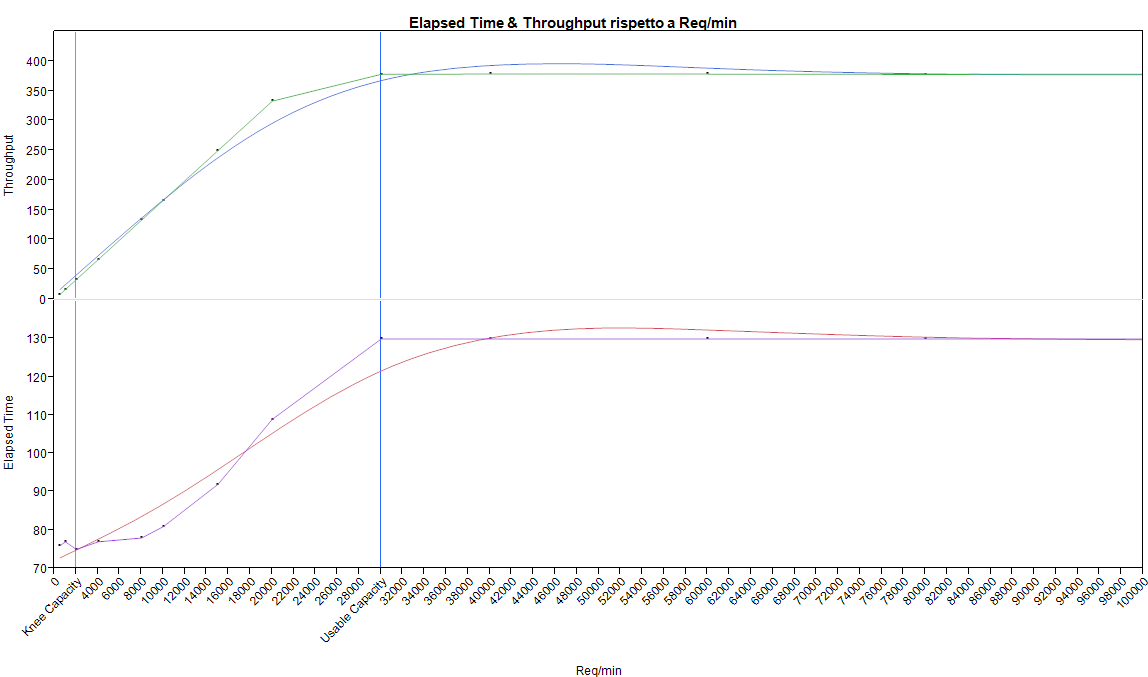
\includegraphics[width=\linewidth, keepaspectratio]{usable_knee_medium}
  \caption{Capacity: Knee (2000 Req/min) / Usable (30000 Req/min)}
\end{figure}

\clearpage

\subsection{Test pagine HTML grandi}
In questo caso sono state utilizzate esclusivamente le richieste HTTP per le pagine
\textit{big\_text} e \textit{big\_image}.\\
In \figurename~\ref{webserver_big_page_summary_report} sono presenti gli esiti del
Summary Report di JMeter.\\

\begin{figure}[!htbp]
  \centering
  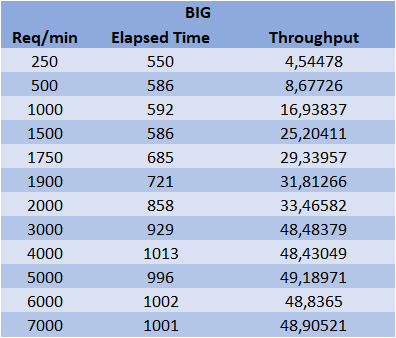
\includegraphics[width=.4\linewidth, keepaspectratio]{capacitytest_big}
  \caption{Test pagine HTML grandi}
  \label{webserver_big_page_summary_report}
\end{figure}

Utilizzando il costruttore di Grafici di \textit{JMP} sono stati analizzati i plot
di Throughput ed Elapsed Time, e definiti i punti di \textit{Knee Capacity} e
\textit{Usable Capacity}.\\

\clearpage

\begin{figure}[!htbp]
  \centering
  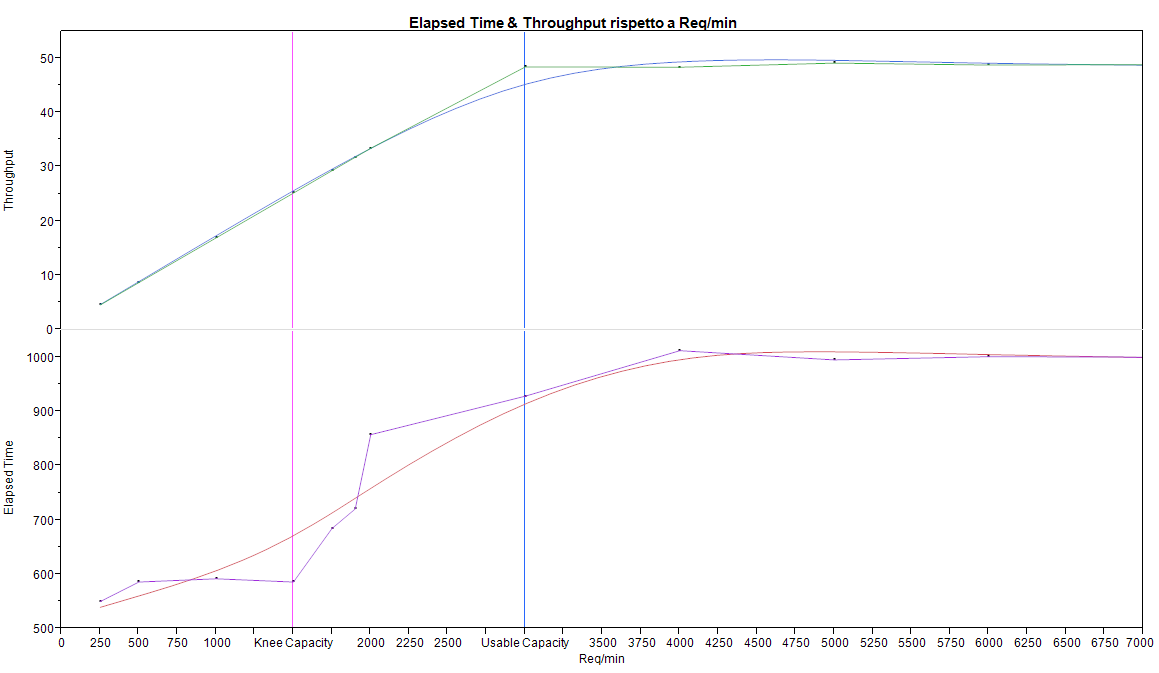
\includegraphics[width=\linewidth, keepaspectratio]{usable_knee_big}
  \caption{Capacity: Knee (1500 Req/min) / Usable (3000 Req/min)}
\end{figure}

\subsection{Test Random}
Finora sono state studiate le capacità di carico del sistema in presenza delle
tre differenti tipologie di pagine HTML disponibili.\\
Dai test effettuati è possibile ricavare il caso medio e il caso peggiore per
ognuno dei punti di funzionamento considerati:
\begin{itemize}
  \item Caso Medio:
  \begin{itemize}
    \item \textbf{Knee Capacity} - 6167
    \item \textbf{Usable Capacity} - 31000
  \end{itemize}
  \item Caso Peggiore:
  \begin{itemize}
    \item \textbf{Knee Capacity} - 1500
    \item \textbf{Usable Capacity} - 3000
  \end{itemize}
\end{itemize}

Come era possibile aspettarsi, il caso peggiore corrisponde esattamente all'uso
delle pagine HTML grandi.\\

Per verificare il reale comportamento del sistema, è stato effettuato un ulteriore
capacity test per definire i punti di funzionamento nel caso di un Random Controller
che genera, in maniera uniforme, richieste HTTP relative a tutte le tipologie di
pagine.\\

In \figurename~\ref{webserver_random_page_summary_report} sono presenti gli esiti del
Summary Report di JMeter.\\

\begin{figure}[!htbp]
  \centering
  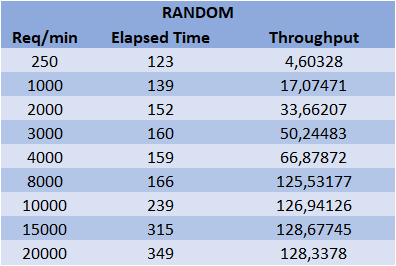
\includegraphics[width=.4\linewidth, keepaspectratio]{capacitytest_random}
  \caption{Test pagine random}
  \label{webserver_random_page_summary_report}
\end{figure}

Utilizzando il costruttore di Grafici di \textit{JMP} sono stati analizzati i plot
di Throughput ed Elapsed Time, e definiti i punti di \textit{Knee Capacity} e
\textit{Usable Capacity}.\\

\begin{figure}[!htbp]
  \centering
  \includegraphics[width=\linewidth, keepaspectratio]{usable_knee_random}
  \caption{Capacity: Knee (2000 Req/min) / Usable (8000 Req/min)}
\end{figure}

\clearpage

\section{Design of Experiments}
Scopo ultimo del DOE è riuscire ad ottenere un design tale da
massimizzare le informazioni ottenute, minimizzando il numero di esperimenti
necessari.\\
Una corretta analisi degli esperimenti aiuta anche a separare gli effetti dei
vari fattori che potrebbero influenzare le prestazioni, determinando se un fattore
è \textit{significativo} oppure se le differenze osservate dipendono semplicemente
da variazioni casuali dovute ad errori di misura e/o parametri non controllabili.\\
Inoltre, il design of experiments è fondamentale anche per ridurre il numero di
esperimenti, quindi il costo, necessari al testing del sistema.\\
Per fare ciò è stata utilizzata la funzionalità \textit{Piano Fattoriale Completo},
resa disponibile dal tool JMP e configurata come in figura \ref{webserver_piano_fattoriale_completo}.\\

\begin{figure}[!htbp]
  \centering
  \includegraphics[width=.9\linewidth, keepaspectratio]{doe_setup}
  \caption{Piano Fattoriale Completo}
  \label{webserver_piano_fattoriale_completo}
\end{figure}

\clearpage

Nel piano fattoriale completo sono stati utilizzati come risposta di interesse,
l'\textit{Average Response Time}(tempo medio di risposta), come fattori il
\textit{Page Size}(categorico a 3 livelli) ed il \textit{Request Rate}(categorico
 a 4 livelli).\\
Il request rate è stato calcolato in funzione della dimensione della pagina,
ed è in particolare definito su 4 livelli:
\begin{itemize}
  \item \textbf{Low} - 20\% della usable capacity
  \item \textbf{Low-Mid} - 40\% della usable capacity
  \item \textbf{High-Mid} - 60\% della usable capacity
  \item \textbf{High} - 80\% della usable capacity
\end{itemize}

In figura \ref{webserver_fattori} sono riportate le capacità usate per ogni dimensione di
pagina e per ogni categoria di carico.\\

\begin{figure}[!htbp]
  \centering
  \includegraphics[width=.7\linewidth, keepaspectratio]{fattori}
  \caption{Req/min al variare del carico e della tipologia di pagina}
  \label{webserver_fattori}
\end{figure}

\clearpage

\subsection{Modello}
In seguito ai 120 esperimenti effettuati è possibile stimare il modello ottenuto.\\
Fare ciò in JMP è molto semplice grazie alla funzionalità \textit{Stima Modello},
riportata in figura \ref{webserver_stima_modello}

\begin{figure}[!htbp]
  \centering
  \includegraphics[width=.6\linewidth, keepaspectratio]{stima_modello}
  \caption{Stima del modello ottenuto}
  \label{webserver_stima_modello}
\end{figure}

Osservando il \textbf{coefficiente di determinazione}($R^{2}$) è possibile
immediatamente affermare che il modello effettua un ottimo fitting dei dati.\\
Infatti il modello spiega circa il 99.8\% della devianza totale.\\
Nell'analisi della varianza riportata in figura \ref{webserver_stima_modello} è possibile anche
osservare che il modello ottenuto è significativo con un livello di confidenza
del 95\%, essendo il test di Fisher rigettato con un $p-value<0.001$.\\

\subsection{Importanza e Significatività Statistica dei fattori}
Importanza e Significatività sono 2 concetti utili e distinti per l'analisi dei
fattori ed entrambi appartengono alla categoria di tecniche
\textbf{ANOVA}(ANalysis Of VAriance).\\
Un fattore è tanto più \textit{importante} quanto ha un rapporto $\frac{SSA}{SST}$
elevato.\\
Un fattore importante non necessariamente è significativo, infatti nella significatività
entrano in gioco anche i \textbf{gradi di libertà}.\\
La significatività di un fattore può anche essere vista come la robustezza del
modello rispetto all'errore e può essere studiata utilizzando un test sulla
varianza.\\

\subsubsection{Importanza}
In figura \ref{webserver_importanza_fattori} sono riportati i valori di importanza dei due
fattori in studio.

\begin{figure}[!htbp]
  \centering
  \includegraphics[width=.9\linewidth, keepaspectratio]{importanza_fattori}
  \caption{Importanza dei Fattori}
  \label{webserver_importanza_fattori}
\end{figure}

Come si evince dalla tabella, il fattore più importante è il \textbf{Page Size},
essendo quello che incide maggiormente sull'elapsed time.\\
Inoltre l'errore risulta essere molto basso, a verifica di quanto affermato dal
coefficiente di determinazione.\\

\clearpage

\subsubsection{Significatività Statistica}
L'analisi della significatività statistica dei fattori basata su ANOVA richiede
che due forti assunzioni siano soddisfatte: \textbf{Normalità} ed
\textbf{Omoschedasticità}.\\
Nel caso in cui una delle due, o entrambe le assunzioni, non siano soddisfatte, è
possibile fare ausilio di ulteriori tecniche e test non parametrici per analizzare
la significatività dei fattori.\\

\subsubsection*{Normalità}
La normalità è studiata sui residui relativi al modello, ottenibili semplicemente
in JMP dalla scheda di \textit{Stima del Modello}.\\
In figura \ref{webserver_normalita} è riportata la distribuzione dei residui ed il test
di \textit{Shapiro-Wilk} per la normalità su un campione di $N<2000$ esperimenti.\\
Il test suggerisce un $p-value<0.001$, quindi l'ipotesi di normalità è rigettata
con il 95\% di confidenza.\\

\begin{figure}[!htbp]
  \centering
  \includegraphics[width=\linewidth, keepaspectratio]{normalita}
  \caption{Normalità dei residui del modello stimato}
  \label{webserver_normalita}
\end{figure}

\clearpage

\subsubsection*{Omoschedasticità}
L'omoschedasticità è studiata sui residui del modello un fattore per volta,
essendo essa la proprietà di costanza della varianza, al variare dei livelli di
ogni singolo fattore.\\
Per fare ciò in JMP, non è studiata la distribuzione dei residui,
ma è effettuata una \textit{Stima Y rispetto X}, per ciascun fattore.\\
In figura \ref{webserver_omoschedasticita} è possibile osservare che il test di \textbf{Levene},
scelto per analizzare l'omoschedasticità dei residui rispetto ai singoli fattori,
dà risultato negativo, rigettando l'ipotesi nulla in entrambi i casi.\\
\'E stato scelto in particolare il test di Levene e non altri per la sua
robustezza a situazioni di non normalità dei dati.\\

\begin{figure}[!htbp]
  \centering
  \includegraphics[width=\linewidth, keepaspectratio]{omoschedasticita}
  \caption{Omoschedasticità dei residui rispetto ai fattori}
  \label{webserver_omoschedasticita}
\end{figure}

\clearpage

Avendo stabilito che il modello stimato non soddisfa le assunzioni di normalità e
omoschedasticità, non è possibile utilizzare l'ANOVA classico con il Fisher-Test
per studiare la significatività dei fattori, bensì il \textit{Kruskal-Wallis Test}.\\

In figura \ref{webserver_kruskal_wallis_significativita} si osservano gli esiti del test
di significatività effettuato su entrambi i fattori.\\
Come da attesa, il fattore \textit{Page Size} è molto significativo,
essendo l'ipotesi nulla pienamente rigettata.\\
Il fattore \textit{Request Rate}, viceversa, è meno significativo
del Page Size, non potendo essere rigettata l'ipotesi nulla con il 95\% di
confidenza, ma solo con il 90\% circa.\\

\begin{figure}[!htbp]
  \centering
  \includegraphics[width=\linewidth, keepaspectratio]{kruskal_wallis_significativita}
  \caption{Kruskal-Wallis Test per la significatività dei fattori}
  \label{webserver_kruskal_wallis_significativita}
\end{figure}


\end{document}
